%%%%%%%%%%%%%%%%%%%%%%%%%%%%%%%%%%%%%%%%%
% Short Sectioned Assignment LaTeX Template Version 1.0 (5/5/12)
% This template has been downloaded from: http://www.LaTeXTemplates.com
% Original author:  Frits Wenneker (http://www.howtotex.com)
% License: CC BY-NC-SA 3.0 (http://creativecommons.org/licenses/by-nc-sa/3.0/)
%%%%%%%%%%%%%%%%%%%%%%%%%%%%%%%%%%%%%%%%%

% \documentclass[paper=a4, fontsize=11pt]{scrartcl} % A4 paper and 11pt font size
\documentclass[11pt, a4paper, fleqn]{report}
\usepackage[T1]{fontenc} % Use 8-bit encoding that has 256 glyphs
\usepackage[utf8]{inputenc}
\usepackage{listings} % para insertar código con formato similar al editor
\usepackage{color}

\definecolor{dkgreen}{rgb}{0,0.6,0}
\definecolor{gray}{rgb}{0.5,0.5,0.5}
\definecolor{mauve}{rgb}{0.58,0,0.82}

\lstset{frame=tb,
	language=python,
	aboveskip=3mm,
	belowskip=3mm,
	showstringspaces=false,
	columns=flexible,
	basicstyle={\small\ttfamily},
	numbers=none,
	numberstyle=\tiny\color{gray},
	keywordstyle=\color{blue},
	commentstyle=\color{dkgreen},
	stringstyle=\color{mauve},
	breaklines=true,
	breakatwhitespace=true,
	tabsize=4
}
\usepackage[spanish, es-tabla]{babel} % Selecciona el español para palabras introducidas automáticamente, p.ej. "septiembre" en la fecha y especifica que se use la palabra Tabla en vez de Cuadro
\usepackage{url} % ,href} %para incluir URLs e hipervínculos dentro del texto (aunque hay que instalar href)
\usepackage{graphics,graphicx, float} %para incluir imágenes y colocarlas
\usepackage[gen]{eurosym} %para incluir el símbolo del euro
\usepackage{cite} %para incluir citas del archivo <nombre>.bib
\usepackage{enumerate}
\usepackage{hyperref}
\usepackage{graphicx}
\usepackage{tabularx}
\usepackage{booktabs}
\usepackage{amsmath}
\graphicspath{{././img}}
\usepackage[table,xcdraw]{xcolor}
\hypersetup{
	colorlinks=true,	% false: boxed links; true: colored links
	linkcolor=blue,  	% color of internal links
	urlcolor=cyan		% color of external links
}
\renewcommand{\familydefault}{\sfdefault}
\usepackage{fancyhdr} % Custom headers and footers
\pagestyle{fancyplain} % Makes all pages in the document conform to the custom headers and footers
\fancyhead[L]{} % Empty left header
\fancyhead[C]{} % Empty center header
\fancyhead[R]{Antonio Manuel Fresneda} % My name
\fancyfoot[L]{} % Empty left footer
\fancyfoot[C]{} % Empty center footer
\fancyfoot[R]{\thepage} % Page numbering for right footer
%\renewcommand{\headrulewidth}{0pt} % Remove header underlines
\renewcommand{\footrulewidth}{0pt} % Remove footer underlines
\setlength{\headheight}{13.6pt} % Customize the height of the header

\definecolor{gray75}{gray}{0.75}
\newcommand{\hsp}{\hspace{20pt}}

\setcounter{secnumdepth}{4}

\begin{document}
	\begin{titlepage}
\newlength{\centeroffset}
\setlength{\centeroffset}{-0.5\oddsidemargin}
\addtolength{\centeroffset}{0.5\evensidemargin}
\thispagestyle{empty}

\noindent\hspace*{\centeroffset}\begin{minipage}{\textwidth}

\centering

\includegraphics[width=0.9\textwidth]{logos/logo_ugr.jpg}\\[1.4cm]

\textsc{ \Large TRABAJO FIN DE GRADO\\[0.2cm]}
\textsc{ GRADO EN INGENIERIA INFORMATICA}\\[1cm]

{\Huge\bfseries   Titulo\\}
\noindent\rule[-1ex]{\textwidth}{3pt}\\[3.5ex]
{\large\bfseries }
\end{minipage}

\vspace{2.5cm}
\noindent\hspace*{\centeroffset}
\begin{minipage}{\textwidth}
\centering

\textbf{Autor}\\ {Antonio Manuel Fresneda Rodríguez}\\[2.5ex]
\textbf{Director}\\ {Salvador García López }\\[2cm]

\includegraphics[width=0.3\textwidth]{logos/etsiit_logo.png}\\[0.1cm]
\textsc{Escuela Técnica Superior de Ingenierías Informática y de Telecomunicación}\\
\textsc{---}\\
Granada, mes de año
\end{minipage}
\end{titlepage}

	\thispagestyle{empty}

\begin{center}
{\large\bfseries Análisis de la intención de emprendimiento a través de una recogida de datos por encuestas mediante técnicas de preprocesamiento de datos y aprendizaje automático.}\\
\end{center}
\begin{center}
Antonio Manuel Fresneda Rodríguez.\\
\end{center}

%\vspace{0.7cm}

\vspace{0.5cm}
\noindent{\textbf{Palabras clave}: \textit{intención emprendedora}, \textit{aprendizaje automático}, \textit{clasificación ordinal}, \textit{clasificación multi-etiqueta}, \textit{regresión}, \textit{Python}
\vspace{0.7cm}

\noindent{\textbf{Resumen}\\
	\linebreak 
	Para que un país sea sólido económicamente, necesita empresas productivas, ya que son las que crean puestos de trabajo e impulsan el desarrollo económico.\\
	Por este motivo, detectar a aquellas personas que son capaces de crear nuevas empresa y promover que estas sean capaces de emprender y facilitar el acceso a recursos y asesoramiento necesarios puede ser un factor importante de cara al crecimiento económico de un país.\\
	La intención emprendedora se puede definir como el estado mental que provoca una atención, experiencia y acción hacia un concepto de negocio, asumiendo que esa persona no reacciona de forma automática antes los estímulos del medio, sino que procesa la información que le rodea (Bird. 1998).\\
	\linebreak
	Resolver este tipo de problemas usando técnicas clásicas puede no ser la mejor opción, ya que puede llegar a ser muy costoso en tiempo y recursos. Con el objetivo de facilitar este tipo de problemas nació el Aprendizaje Automático.\\
	El Aprendizaje Automático hace uso de unos \textbf{datos} y construye un \textbf{modelo} capaz de realizar \textbf{predicciones} tanto de los datos que ha usado como de datos nuevos.\\
	Este campo ha sufrido una gran evolución en estos últimos años, donde se han propuesto nuevos problemas, modelos y metodología, aumentando la cantidad de problemas que pueden ser resueltos.\\
	\linebreak
	Este trabajo hace uso de técnicas de Aprendizaje Automático y de unos \textbf{datos} recogidos sobre un conjunto de la población española y ecuatoriana para intentar predecir si una persona va a tener una intención emprendedora y cuales son los factores más importantes para que una persona tome este tipo de decisiones.
\cleardoublepage

\begin{center}
	{\large\bfseries Analysis of entrepreneurial intention through data collected by surveys using data preprocessing techniques and Machine Learning }\\
\end{center}
\begin{center}
	Antonio Manuel Fresneda Rodríguez\\
\end{center}
\vspace{0.5cm}
\noindent{\textbf{Keywords}: \textit{entrepreneurial intention}, \textit{machine learning}, \textit{ordinal classification}, \textit{multi-label clasification}, \textit{regression}, \textit{Python}
\vspace{0.7cm}

\noindent{\textbf{Abstract}\\
\linebreak
To keep a country solid economically, it will need profitable companies, as these are in charge of creating job posts and pushing the economic growth.\\
For these reasons, detecting people capable of creating new companies and helping them to get the resources and advice, can be important for the economic growth of a country.
Entrepreneurial intention is the mental state of mind that precedes action and directs attention toward entrepreneurial behaviors such as starting a new business. This person will use all the information around him/her and will process it to get the best decision, instead of reacting automatically to the stimuli (Bird 1998).\\
\linebreak
Solving this kind of problem using classic techniques may not be the best choice, as this can be time and resource-intensive. The goal of  Machine Learning is to ease this kind of problem. This approach will use data to build a mathematical model that will predict the data used to create the model and, most important, new data that the model hasn't used.
This field has evolved significantly during the last years, proposing new problems, models, and methodology.\\
\linebreak
This work will use Machine Learning techniques and data collected from Spanish and Ecuadorian people to find the entrepreneurial intention of a person and which are the key factors that make that choice.
\cleardoublepage
\chapter*{}
\thispagestyle{empty}

\noindent\rule[-1ex]{\textwidth}{2pt}\\[4.5ex]

Yo, \textbf{Antonio Manuel Fresneda Rodríguez}, alumno de la titulación Ingeniería Informática de la \textbf{Escuela Técnica Superior de Ingenierías Informática y de Telecomunicación de la Universidad de Granada}, con DNI 77447672W, autorizo la ubicación de la siguiente copia de mi Trabajo Fin de Grado en la biblioteca del centro para que pueda ser consultada por las personas que lo deseen.
\vspace{6cm}

\noindent Fdo: Antonio Manuel Fresneda Rodríguez
\vspace{2cm}
\begin{flushright}
	Granada a 17 de Noviembre de 2021 .
\end{flushright}

\cleardoublepage
\thispagestyle{empty}

\noindent\rule[-1ex]{\textwidth}{2pt}\\[4.5ex]

D. \textbf{Salvador García López}, Profesor del Área de Computación y Sistemas Inteligentes del Departamento de Ciencias de la Computación e Inteligencia Artificial de la Universidad de Granada.

\vspace{0.5cm}

\textbf{Informo:}

\vspace{0.5cm}

Que el presente trabajo, titulado \textit{\textbf{ Análisis de la intención de emprendimiento a través de una recogida de datos por encuestas mediante técnicas de preprocesamiento de datos y aprendizaje automático}},
ha sido realizado bajo mi supervisión por \textbf{Antonio Manuel Fresneda Rodríguez}, y autorizo la defensa de dicho trabajo ante el tribunal
que corresponda.

\vspace{0.5cm}

Y para que conste, expiden y firman el presente informe en Granada a Noviembre de 2021.

\vspace{1cm}

\textbf{El/la director(a)/es: }

\vspace{5cm}

\noindent \textbf{Salvador García López}
\pagebreak
\section*{Agradecimientos}
Me gustaría comenzar esta sección agradeciendo a mis padres el esfuerzo y la oportunidad que ellos no tuvieron para disfrutar de una educación universitaria. Muchas gracias por todo y os estoy realmente agradecido. \\
A mis hermanas, que son muy importantes para mi y que siempre han estado ahí para apoyarme y de vez en cuando para cabrearme también.
A toda mi familia, gracias abuela, abuelo, tíos, tías, primos, primas os quiero mucho y sois el pilar más importante de mi vida.\\
\linebreak
No me quiero olvidar tampoco de aquellos profesores que han formado parte en mi educación, desde la secundaria, donde creo que en ese momento no llegué a valorar lo importante que era la formación en ingles que estuve recibiendo, hasta todos aquellos docentes que me han dado clase durante todos estos años en la ETSIIT aprendiendo todo lo que me ha llevado a conseguir un trabajo en estas épocas tan complicadas y que me está haciendo muy feliz. Muchas gracias.\\
Una mención aparte para Salva, que me ha propuesto un trabajo muy interesante, me ha ayudado y animado a realizar este trabajo al que le he dedicado un montón de horas en estos meses. Muchas gracias.\\
\linebreak
Agradecer también a todos mis amigos y amigas que he estado haciendo durante todos estos años, muchas gracias por estar siempre ahí y por ser capaces de hacerme desconectar de vez en cuando. 

	\newpage
	\tableofcontents
	\pagebreak

	\chapter{Introducción}
Gracias a la evolución tecnológica que hemos experimentado estos últimos años, y sobre todo a la gigantesca expansión del Internet y  a la cantidad de datos generados por dispositivos conectados a la red, ha provocado un enorme interés analizar los datos recogidos.\\
Gracias a esta información es los que nos identifican como posibles compradores de un producto, los que hacen que los coches puedan conducir por si mismos o incluso, ayuden al personal médico detectar una patología a partir de ciertos datos del paciente.
\linebreak
Se denomina \textbf{ciencia de datos} a la extracción del conocimiento de una gran cantidad datos mediante el uso del software y de  técnicas estadísticas. Este conocimiento puede ser usado para \textbf{predecir} cierta salida en función de los datos, para \textbf{detectar grupos} de datos que tengan características similares, \textbf{explicar} el comportamiento de esos datos, entre otros muchos más casos de uso. \\
\linebreak
El \textbf{Machine Learning} es un campo dentro de la ciencia de datos que se centra en la creación y entrenamiento de modelos de predicción con el objetivo de minimizar el error de salida ante una nueva entrada que el modelo no ha usado en la fase de entrenamiento.
\section{Machine Learning}
El \textbf{Machine Learning} (aprendizaje automático) es un campo de la Inteligencia Artificial que se centra en el desarrollo de técnicas que permitan a las computadores extraer conocimiento a partir de unos datos.\\
\linebreak
Estos datos pueden estar definidos de una gran número de formas, observaciones recogidas por sensores, imágenes, valoraciones de usuarios, etc. En el caso particular de este trabajo en el que se enfoca este proyecto, el \textbf{conjunto de datos} con el que se va a trabajar tiene una cantidad de \textbf{muestras} en la que cada muestra tiene un número fijo de \textbf{características} que identifican a cada muestra. Además, el conjunto de datos con el que se está trabajando, contiene una serie de \textbf{etiquetas} asignada a cada muestra.\\
\linebreak
 Usando la naturaleza de los datos, se pueden dividir los distintos tipos de técnicas que se usan en ML.
\subsection{Agrupamiento en función de los datos disponibles}
Se puede usar la naturaleza de los datos para definir varios tipos de algoritmos, ya que la metodología a seguir cuando se trabaja con datos \textbf{etiquetados} o con datos sin etiquetar es distinta. Usando esta idea, las técnicas usadas en ML pueden ser agrupadas en \textbf{aprendizaje supervisado}, \textbf{no supervisado} ó \textbf{semi-supervisado}:
\begin{itemize}
	\item \textbf{Aprendizaje supervisado:} Este conjunto de técnicas se caracteriza debido a que cada muestra tiene una ó más \textbf{etiquetas}(variable/s objetivo) y tiene como finalidad hacer uso de las características de cada muestra para \textbf{predecir} las variables objetivo de nuevas muestras que no pertenecen al conjunto de datos inicial. Alguna de las tareas que entran dentro de este grupo son \textbf{Clasificación} ó \textbf{Regresión}
	\item \textbf{Aprendizaje no supervisado:} A diferencia del anterior, las técnicas de aprendizaje no supervisado se diferencian en que las muestras \textbf{no están etiquetadas}, por lo que no se puede \textbf{predecir} ninguna variable. Estas técnicas se caracterizan por ser capaces de \textbf{reconocer patrones} dentro del conjunto de datos, etiquetando las nuevas entradas haciendo uso de ellos. La tarea más común es \textbf{Clustering}
\end{itemize}
Anteriormente se han mencionado tareas como \textbf{clasificación}, \textbf{regresión} o \textbf{clustering}, en la siguiente sección se va a profundizar más, explicando en que consiste cada una y que objetivos tienen.
\subsection{Agrupamiento en función de la tarea}
\begin{itemize}
		 \item \textbf{Clasificación:} Como se mencionó previamente, esta tarea tiene sentido cuando se usa un conjunto de datos que está etiquetado. El objetivo principal de clasificación consiste en dada una nueva muestra, \textbf{predecir} una o varias etiquetas en función del conjunto de datos que se ha usado. Estas etiquetas suelen ser variables \textbf{discretas}
		 \item \textbf{Regresión:} A diferencia de clasificación, donde las variables objetivo son discretas, en este caso las variables objetivo son continuas. El propósito de estas técnicas es el de predecir un \textbf{valor} para nuevas muestras.
		 \item \textbf{Clustering:} El objetivo es el de detección de patrones usando datos no etiquetados.
\end{itemize}
Dentro de las tareas de clasificación, se pueden dividir en varios grupos. En la siguiente sección se va a explicar los distintos tipos de clasificación, ya que ayudara a entender la naturaleza del problema que se esta tratando en este trabajo.
\section{Tipos de clasificación}
Como ya se ha mencionado previamente, clasificación usa un conjunto de datos para predecir un valor de una o mas variables de salida. Según el tipo de variable que se va a predecir, se pueden identificar los siguientes tipos de clasificación:
\subsection*{Clasificación binaria}
Este es el tipo de clasificación más sencilla, ya que la variable objetivo solo va a tener dos posibles valores. Estos valores se conocen como clase positiva (1) ó clase negativa (0). De aquí viene el nombre de clasificación \textbf{binaria}, ya que la variable objetivo es binaria.\\
Ejemplos de este tipo de clasificación son detectar si un mensaje es spam, si en función de ciertos valores una bomba de agua puede fallar, o detectar si un cliente de un banco va a tener deudas usando ciertos parámetros.
\begin{figure}[H]
	\centering
	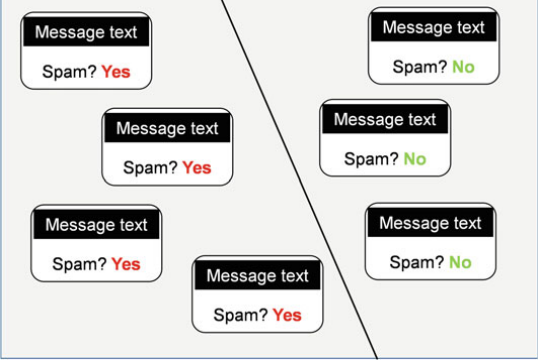
\includegraphics[scale=0.4]{binary-class.png}
	\caption{Ejemplo de clasificación binaria: Identificar si un correo electrónico es spam.}
	\label{fig:bclass}
\end{figure}
\subsection*{Clasificación multi-clase}
Los conjuntos de datos que se usan en clasificación multi-clase son una generalización del caso de clasificación binaria, ya que al igual que la clasificación binaria, solo existe una única variable objetivo, siendo la principal diferencia que la variable objetivo puede tener cualquier valor dentro de un conjunto de posibles valores. Es importante destacar que estos valores son \textbf{discretos} y \textbf{finitos}. El ejemplo más conocido de este tipo de clasificación es la \textbf{clasificación de la flor del Iris}, donde en función de la longitud y anchura del sépalo y del pétalo, se predice si la flor es setosa, virgínica o versicolor.
\begin{figure}[H]
	\centering
	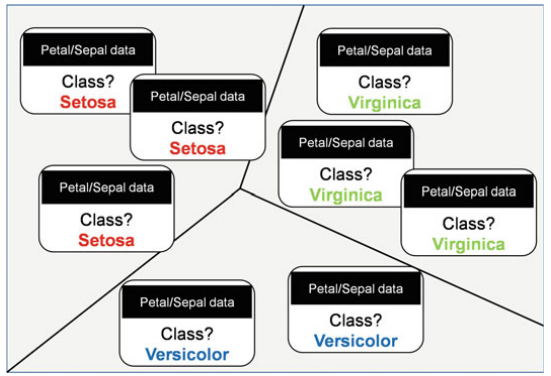
\includegraphics[scale=0.4]{multiclass-class.png}
	\caption{Ejemplo de clasificación multi-clase: Clasificación de la flor del Iris}
	\label{fig:mcclass}
\end{figure}
\subsection*{Clasificación ordinal}
Clasificación ordinal es un caso particular de clasificación multi-clase donde existe una relación de orden entre las clases.\\
Un ejemplo de este tipo de clasificación es el de predecir la valoración de una película, predecir las preferencias de una persona (en desacuerdo, de acuerdo).
\subsection*{Clasificación multi-etiqueta}
A diferencia de los anteriores tipos de clasificación, cada muestra tiene un \textbf{conjunto de variables objetivo} en lugar de una única variable. En este caso, el número de variables objetivo es fijo, siendo estas de tipo binario. A cada combinación distinta de valores se conoce como \textit{labelset}.\\
Los algoritmos que usados para este tipo de problema deben de ser capaces de realizar varias predicciones, ya sea modificando los datos originales o adaptando algoritmos de clasificación binaria o multi-clase.\\
\linebreak
Un ejemplo de este tipo de clasificación puede ser el de comprobar si una imagen contiene ciertos elementos. 
\begin{figure}[H]
	\centering
	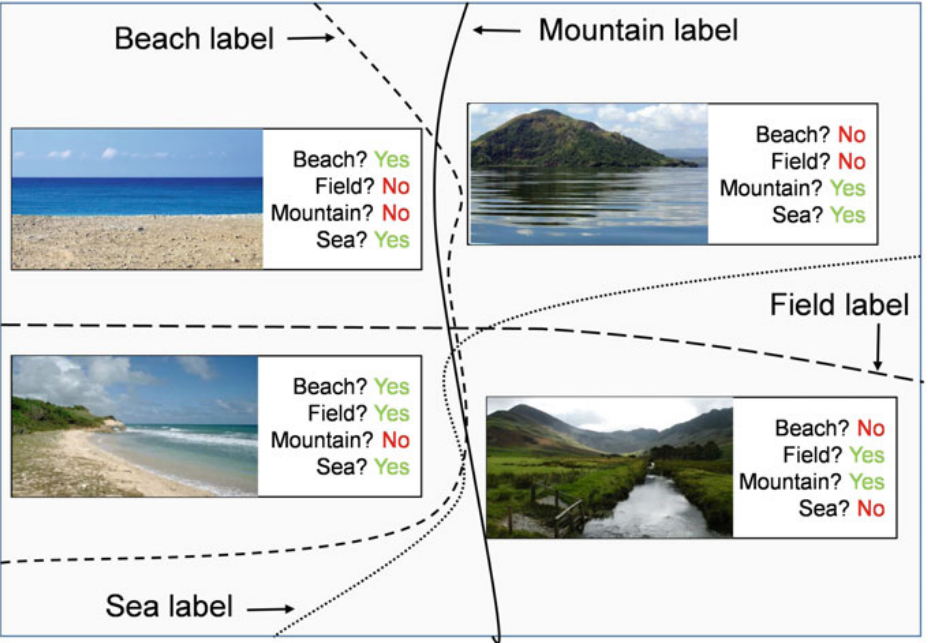
\includegraphics[scale=0.4]{multilabel-class.png}
	\caption{Ejemplo de clasificación multi-etiqueta: Clasificar si una imagen contiene ciertos elementos.}
	\label{fig:mlclasss}
\end{figure}
\subsection*{Clasificación multi-dimensional}
Al igual que la clasificación multi-clase es una generalización del caso binario, la clasificación multi-dimensional es una generalización de la clasificación multi-etiqueta.\\
En este caso, cada muestra tiene un conjunto fijo de variables objetivo que pueden tomar cualquier valor dentro de un conjunto de posibles valores. 
\section{Introducción al problema}
Pongámonos en situación de una persona dentro del departamento de marketing de una empresa que se centra en la creación de cursos. Determinar que variables son capaces de definir la intención emprendedora de una sección de la población podría ser beneficioso para la empresa, ya que podrían crear esos cursos enfocándose en aquellas variables más importantes (edad, estudios, ......) para que de una forma más eficiente captar a interesados, cambiar ciertas características de esos cursos para que sean accesibles a gente con más interés y, en definitiva, optimizar los recursos empleados en esos cursos para incrementar el beneficio.\\

	\pagebreak

	\section{Pre-procesamiento}
\subsection{Introducción}
Cualquier problema en ciencia de datos, comienza con un estudio exhaustivo de los datos proporcionados y realizar un \textbf{procesamiento} previo.
Si este paso es omitido, los algoritmos no se comportarán de forma óptima, debido a  que van a lidiar con unos datos que tendrán valores perdidos, que no estén normalizados, datos des-balanceados, irrelevantes, entre otras problemas. El objetivo de esta fase, es realizar ciertas transformaciones sobres los datos en bruto filtrando esta información para que los algoritmos no tengan que enfrentarse a estos problemas.
\subsection{Análisis exploratorio de los datos}
Para comenzar, se empezó leyendo la documentación aportada con los datos, la cual contenía los siguientes campos:
\begin{itemize}
	\item \textbf{Nombre:} Nombre de la característica.
	\item \textbf{Descripción:} Breve resumen explicando el origen de la característica o el enunciado de la pregunta en la encuesta.
	\item \textbf{Valores:} Tipo y/o rango que toma la característica.
\end{itemize}

Esta información es muy útil, ya que aparte de darnos un poco más de conocimiento del objetivo que queremos alcanzar con estos datos, nos da información de algunas características redundantes.

\begin{table}[H]
	\begin{tabular}{|l|l|l|}
		\cline{1-3}
		CF9  &	Normalmente es posible reducir...&	Respuesta: Verdadera/Falsa. \\ \cline{1-3}
		QF9	& Variable creada a partir de CF9.  & Valor 1 si la respuesta es correcta, 0 si no. \\ \cline{1-3}
	\end{tabular}
	\label{tab:columnas_iguales}
	\caption{Comparación de dos características redundantes.}
\end{table}
Como podemos ver, estas dos columnas contienen información redundante, ya que siendo una respuesta de tipo verdadero o falso, tenemos dos columnas con la misma información. Este caso se repite en varios casos, y en todos ellos se ha optado por dejar unicamente la que tiene los valores numéricos.\\
\linebreak
El siguiente paso ha sido el de obtener las columnas que se van a usar como predictores.
La peculiaridad de este conjunto de datos tenemos 7 columnas que van a ser las que los algoritmos tienen que intentar predecir. De estas 7 columnas tenemos 6 de ellas que son de tipo ordinal, almacenando la opinión (en escala Likert) que ha tenido el entrevistado sobre la pregunta en concreto. La ultima de estas columnas es la media de las 6 columnas.\\
 A continuación se muestra una tabla con la ocurrencia de cada valor para las columnas que vamos a usar:\\
\linebreak
 \begin{figure}[H]
 	 \centering
	 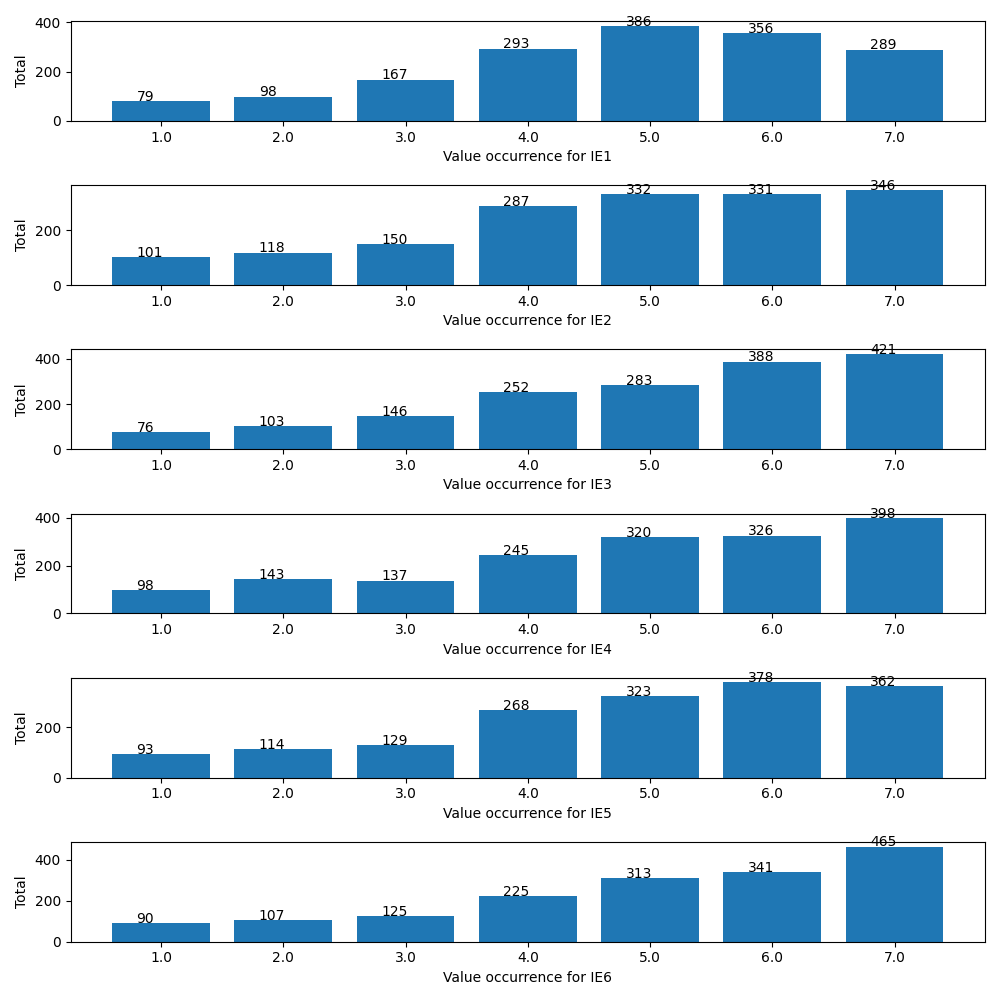
\includegraphics[scale=0.5]{src/value_occurrences.png}
	\caption{Conteo de valores para las columnas usadas como predictores}
	\label{tab:ocurrencia_valores}
\end{figure}
Una vez leída esta documentación y detectados algunos casos de columnas con información redundante, se cargaron los datos y se sacaron una serie de métricas. Estamos ante un conjunto de datos formados por un total de 1672 ejemplos y con 246 características (antes de realizar cualquier tipo de procesamiento), las cuales pueden ser de tipo entero, flotante o categóricas.
\pagebreak
\subsection{Pre-procesado de datos}
En este paso también se han borrado aquellas columnas las cuales corresponden a respuestas de tipo abierta. Estas características pueden llegar a contener un valor único por cada uno de los ejemplos que tenemos. En un principio, van a ser descartadas, pero en fases siguientes se podría realizar un procesamiento más exhaustivo sobre dicha columna, agrupando ciertos valores y reduciendo así la complejidad. Cabe destacar que esta información no se esta perdiendo totalmente, ya que tenemos en todos los casos una nueva columna la cual contiene si la persona respondió correctamente o no a dicha pregunta. \\
\linebreak
Un caso particular que se detectó en esta fase, fue el de las características \textbf{BFx} y \textbf{BFxAdaptada} (hay un total de 4 columnas de este tipo). Las primeras columnas de este tipo, solo contenían la respuesta las personas que realizaron la entrevista en un único año, mientras que las columnas del segundo tipo contenían la respuestas de los dos años. Antes de eliminar las columnas del primer tipo, se realizo una comprobación para ver si realmente los datos comunes entre las dos columnas eran los mismos para así asegurar que no se están perdiendo datos.
\linebreak
El siguiente paso, ha sido analizar los valores únicos de cada variable, esto nos permitió detectar valores no validos. Se encontró los siguientes casos de valores nó validos:
\begin{itemize}
	\item \textbf{Valores perdidos especificados como espacios:} Si no procesamos estos valores, el algoritmo puede detectarlo como un valor válido, introduciendo así ruido en el modelo. Estos valores se cambiaron por \textit{NaN}.
	\item \textbf{Valores perdidos especificados como "\textit{No contesta}":} Estos valores se ven sobre todo en columnas con datos ordinales. El enfoque que se ha escogido ha sido el de cambiarlas por \textit{NaN}.
	\item \textbf{Valores inválidos en la columna "\textit{género}":} Según la documentación, los únicos valores que forman esta columna son \textit{hombre} y \textit{mujer}, pero dentro del conjunto de datos se detectan valores como \textit{si} y \textit{no}. No podemos saber si la persona que contestó la encuesta se equivocó ó le llegó una versión distinta de la encuesta, así que, estos valores dentro de la columna \textit{género} se reemplazaron por \textit{NaN}.
	\item \textbf{Valores binarios codificados como strings:} Este caso no es necesariamente un valor no válido, pero se decidió cambiar estos valores binarios codificados como \textit{sí} o \textit{no} por \textit{1} y \textit{0} respectivamente. Con este cambio no vamos a perder información y vamos a ahorrarnos el codificar ciertas columnas en fases posteriores.
\end{itemize}

El siguiente paso ha sido el de obtener las columnas con una alta correlación. Hemos considerado como alta correlación, aquellas columnas cuya correlación sea mayor que 0.9\\
El resultado ha sido: \\
\begin{table}[H]
	\centering
	\begin{tabular}{|l|l|l|l|}
		\cline{1-3}
		Columna 1             & Columna 2              & Correlación  \\ \cline{1-3}
		IF1.6jTiene    	      &  FI\_Insur             &  1.000000    \\ \cline{1-3}
		FinLit total(1-19)    & FinLit normaliz        & 1.000000     \\ \cline{1-3}
		ConFin(1\_7)          & ConFin(1\_8)           &  0.987110    \\ \cline{1-3}
		FinBehSinBorrow (1-6) & FinBeh con borrow(1-7) &  0.948779    \\ \cline{1-3}
	\end{tabular}
	\label{tab:correlacion}
	\caption{Matriz de correlación}
\end{table}
Volviendo a revisar la documentación, tenemos las siguientes descripciones:
\linebreak
\begin{itemize}
	\item \textit{FI\_Insur}: Si tiene Productos de seguro: contrato de seguros (IF1.6jTiene). Valor 1 cuando tiene alguno, en caso contrario toma valor 0.
	 \item \textit{FinLit normaliz}: Puntuación de Competencia financiera normalizada calculado dividiendo entre 19 y multiplicando por 100. Indica el porcentaje de competencia financiera general sobre 100. (columna \textit{FinLit total}).
	 \item \textit{ConFin(1\_7)}: Variable global de Conocimientos financieros generales sumando QF3 a QF9. \textit{ConFin(1\_8)} suma de QF2 a QF9.
	 \item \textit{FinBehSinBorrow (1-6)}: Suma de las variables de comportamiento financiero excepto Borrow. \textit{FinBeh con borrow(1-7) } introduce Borrow.
\end{itemize}
Como vemos, viendo la explicación de las variables, podemos prescindir de ciertas columnas. En este caso se han descartados las características de la columna 2.\\
\linebreak
Por último, se ha dividido el conjunto de datos en los conjuntos de entrenamiento y test.
\linebreak
A continuación, se va a explicar qué algoritmos se han usado para imputación de valores perdidos, codificación de características categóricas y normalización, etc. En cada subsección de \textbf{\ref{sec:algoritmos}-\nameref{sec:algoritmos}}, se especifica que algoritmos han sido aplicados a cada modelo.

\subsubsection{Valores perdidos}
Un valor perdido es aquel para el que en una variable determinada, no consta en una o más muestras de conjunto de datos. En caso de que se trabaje con un conjunto de datos con valores perdidos, se puede optar por:
\begin{itemize}
	\item \textbf{Eliminar} aquellas muestras que contengan valores perdidos.
	\item \textbf{Imputar} los valores perdidos en función de del resto de muestras.
\end{itemize}

La opción de eliminar las muestras tiene la ventaja de que no se está introduciendo información artificial al conjunto de datos, manteniendo así las características originales, pero claramente tiene una desventaja, y es que se está eliminando información, pudiendo impactar en el comportamiento de los algoritmos.\\
\linebreak
La segunda opción implica el estar modificando el conjunto de datos con muestras \textbf{artificiales}, alterando así las características del conjunto de datos pero sin eliminar información.\\
Estas muestras artificiales se pueden usar estadísticos como la \textbf{media}, \textbf{moda} de la variable con valores perdidos. El uso de estos estadísticos en esta fase tiene una gran desventaja: Solo se está usando la información de la propia variable, cabiendo la posibilidad que una o más variables del resto del conjunto de datos influyan en la variable que se está tratando. \\
\linebreak
Para evitar la desventaja del uso de estadísticos, puede usarse un algoritmo de machine learning para \textbf{predecir} que valor tendría el valor perdido de la variable que se está analizando. \\
\linebreak
Para imputar valores perdidos en una primera iteración del proceso, se ha usado el algoritmo KNN. Este algoritmo está explicado con más profundidad en la sección \textbf{\ref{alg:knn}-\nameref{alg:knn}} de este mismo documento, resumiendo, dada una muestra nueva,  este algoritmo calcula la \textbf{diferencia} entre la nueva muestra y \textbf{todas} las muestras del conjunto de datos, seleccionando la variable de salida de las $K$ muestras más cercanas y asignando el valor predicho en función de las variables de salida seleccionadas.
\subsubsection{Codificación de variables categóricas}
Existen algoritmos que no aceptan variables categóricas (Redes Neuronales, KNN, SVM, etc) por lo que un paso muy importante antes de usar estos algoritmos, es de adaptar el conjunto de datos para que el algoritmo funcione. \\
Una opción puede ser eliminar aquellas variables categóricas, pero se podría estar perdiendo información importante. Para usar estos algoritmos sin eliminar información lo más normal es \textbf{codificar} las variables categóricas.\\
Existen dos opciones para la codificación:
\begin{enumerate}
	\item \textbf{Codificación por etiqueta:} Cada valor único de la variable se sustituye por un valor entero.
	\item\textbf{Codificación \textit{one-hot }:} Se cambia la variable categórica por una serie de variables \textit{dummies}
\end{enumerate}

La codificación por etiqueta tiene la ventaja que es la más natural para los humanos y podría parecer suficiente, pero tiene una gran desventaja: Los valores enteros tienen una \textbf{relación de orden} entre cada valor. Los algoritmos de machine learning son capaces de entender esta relación de orden y perjudicar la eficacia del modelo.\\
\linebreak
La codificación \textit{one-hot}  crea una variable por cada valor único de la variable a codificar. Cada nueva variable se asocia con un valor único y tendrá el valor $1$ cuando el valor para esa muestra sea el asociado, fijando el valor a $0$ para el resto de nuevas variables. Un ejemplo sería el siguiente:\\
Dada el siguiente conjunto de datos de ejemplo:\\
\begin{table}[H]
	\centering
	\begin{tabular}{|c|c|}
		\cline{1-2}
		ID    &	  Vehículo.  \\ \cline{1-2}
		0	  &   Moto       \\ \cline{1-2}
		1	  &   Camión     \\ \cline{1-2}
		2     &   Coche      \\ \cline{1-2}
		3	  &   Moto       \\ \cline{1-2}
	\end{tabular}
	\caption{Conjunto de datos de ejemplo.}
	\label{tab:conjunto_ejemplo}
\end{table}
Si usamos codificamos la variable \textit{vehículo} usando la etiqueta, estaríamos imponiendo una relación de orden sobre \textit{moto, camión y coche}, pudiendo "confundir" al algoritmo. Si usamos la codificación \textit{one hot}, el conjunto quedaría:

\begin{table}[H]
	\centering
	\begin{tabular}{|c|c|c|c|}
		\cline{1-4}
		ID  & Vehículo\_moto & Vehículo\_camión & Vehículo\_coche. \\ \cline{1-4}
		0	& 1  			 & 0				& 0		           \\ \cline{1-4}
		1	& 0				 & 1				& 0 			   \\ \cline{1-4}
		2   & 0 			 & 0 				& 1				   \\ \cline{1-4}
		3   & 1 			 & 0 				& 0			       \\ \cline{1-4}
	\end{tabular}
	\caption{Conjunto de datos de ejemplo tras codificar}
	\label{tab:conjunto_ejemplo_cod}
\end{table}
Como se ve en la tabla \ref{tab:conjunto_ejemplo_cod}, se ha transformado la columna \textit{vehículo} en tres columnas distintas, tomando el valor 1 cuando el valor de la variable sin codificar coincide con la variable asignada para ese valor. \\
\linebreak
Este modelo tiene una desventaja clara, y es se van a crear tantas columnas como valores único tenga la variable a codificar, esto puede incrementar significativamente el tamaño del conjunto de datos, pudiendo impactar en el rendimiento de los modelos.

	\pagebreak

	\chapter{ Regresión}
\label{sec:algoritmos}
Como se ha comentado previamente, se está trabajando sobre  un problema bastante peculiar, donde se intenta predecir distintas variables ordinales. Antes de comenzar con algoritmos más complejos, el primer enfoque para resolver el problema ha sido el de usar una media de cada variable a predecir. \\
Es cierto que usando este enfoque, estamos perdiendo información muy importante:  se está suponiendo que todas las variables son igualmente importantes, lo cual es una desventaja de esta aproximación al problema.
Por el contrario, este enfoque tiene la ventaja de estar usando algoritmos clásicos de regresión, proporcionando una salida más general, además de que usando este enfoque primero, descartamos la posibilidad de tener un conjunto de datos con mucho ruido o con un mal muestreo de los datos.\\
\linebreak
En esta sección vamos a explicar que algoritmos se han usado después del pre-procesamiento inicial.\\
Existe un teorema llamado\textbf{\textit{No-Free-Lunch}} que afirma no existe un algoritmo que resuelva los problemas de machine learning mejor que otro. Partiendo de esta idea, el objetivo principal de esta sección es el de comprobar el comportamiento de una serie de modelos e intentar mejorar el rendimiento de los mismos, añadiendo nuevos pasos a la etapa de pre-procesamiento y volviendo a entrenar los modelos que se han seleccionado. \\
\linebreak
\section{Rendimiento de modelos de regresión}
Para comprobar el comportamiento de los distintos modelos seleccionados, se han usado las siguientes \textbf{métricas de regresión}: \textit{\textbf{Coeficiente de determinación}} (se denota como $R^2$), \textit{\textbf{Desviación de Poisson}} y \textit{\textbf{Error cuadrático medio}}
\subsection{Coeficiente de determinación}
Se define como \textbf{coeficiente de determinación} como la proporción de la varianza total explicada por la variables independientes del modelo. Proporciona una indicación de como de bueno es un ajuste y por tanto, una medida de como de bueno es el modelo cuando predice nuevas muestras.\\
\linebreak
Matemáticamente, se define el coeficiente de determinación como:
\[
	R^2 (y, \hat{y}) = 1 - \frac{\sum_{i=1}^{n}(y_i - \hat{y}_i)^2}    {\sum_{i=1}^{n} (y_i - \overline{y})^2}
\]

Donde:
\begin{itemize}
	\item $y$ es el conjunto de valores reales para las variables objetivo.
	\item $\hat{y}$ es el valor predicho para los valores objetivo.
	\item $\hat{y}_i$ es la predicción de la  i-ésima muestra.
	\item $y_i$ es el valor real de la i-ésima muestra.
	\item $\overline{y} = \frac{1}{n} \sum_{i=1}^{n} y_i$.
	\item $n$ es el numero de muestras del conjunto.
\end{itemize}
insertar graficos explicando varianza,  etc
\subsection{Desviación de Poisson}
\subsection{Error cuadrático medio}
El error cuadrático medio de un estimador mide el promedio de los errores al cuadrado.  \\
Matemáticamente, se define el error cuadrático medio como:
\[
	MSE(y,\hat{y}) = \frac{1}{n} \sum_{i=1}^{n} (y_i - \hat{y}_i) ^2
\]
Donde:
\begin{itemize}
	\item $y$ es el conjunto de valores reales para las variables objetivo.
	\item $\hat{y}$ es el valor predicho para los valores objetivo.
	\item $\hat{y}_i$ es la predicción de la  i-ésima muestra.
	\item $y_i$ es el valor real de la i-ésima muestra.
	\item $n$ es el numero de muestras del conjunto.
\end{itemize}
\subsection{Conjuntos de validación}
\label{sec:validation}
Para ver el comportamiento de un modelo, no basta con definir un conjunto de entrenamiento para entrenar el modelo que se ha seleccionado y un conjunto de test para comprobar el comportamiento con datos que el algoritmo no conoce.  Aunque a primera vista esta parece una técnica correcta, tiene varios inconvenientes:
\begin{itemize}
	\item Cuando se ajustan los hiper-parámetros de los modelos,  se podría llegar a ajustar el modelo al conjunto de test, produciendo un sobre-ajuste.
	\item Solo se esta usando una parte de los datos para validar el modelo, nada asegura que el conjunto de test sea representativo del conjunto de datos con el que se está trabajando.
\end{itemize}
Para solventar estas y algunos otros problemas que que tiene esta metodología, se usa la \textbf{validación cruzada}.\\
\linebreak
En lugar de usar el conjunto de entrenamiento para entrenar un único modelo, se divide el conjunto de entrenamiento en $k$ partes, entrenando $k$ modelos usando $k-1$ subconjunto y usando el restante como de test. \\
 \begin{figure}[H]
	\centering
	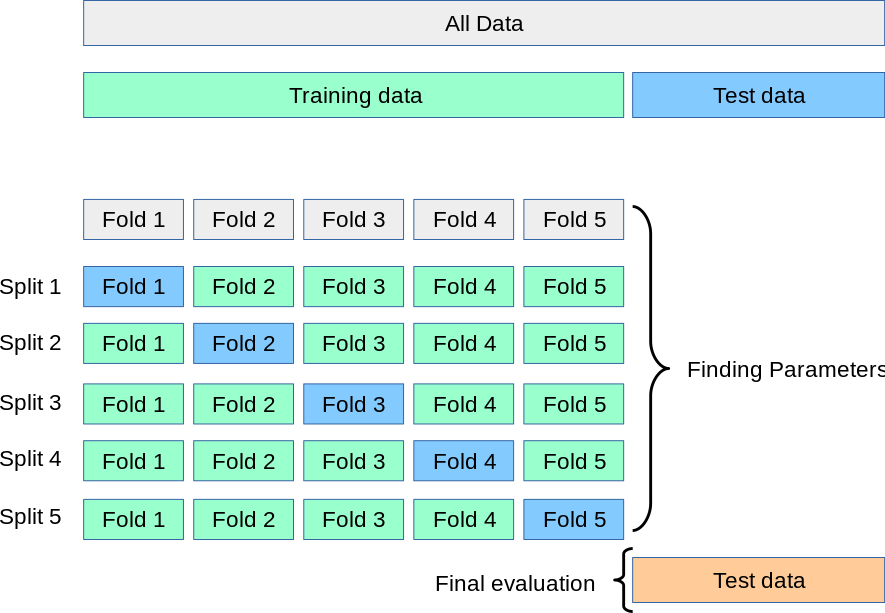
\includegraphics[scale=0.4]{grid_search_cross_validation.png}
	\caption{Ejemplo de validación cruzada con $k=5$}
	\label{fig:cross-validation}
\end{figure}
Como se aprecia en la figura \ref{fig:cross-validation},  se ha dividido el conjunto de datos en 5 conjuntos (folds), usando en cada iteración 4 para entrenar el modelo y uno para verificar con datos que el modelo no ha visto. Finalmente, se usa el conjunto de test (habiendo entrenado previamente el modelo con todo el conjunto de entrenamiento).
\subsection{Gráficos}
Además del uso de las métricas mencionadas previamente, se han creado las siguientes gráficas para visualizar los errores que esta haciendo un modelo en concreto. Esto ayuda a la toma de decisiones en fases siguientes.\\
Las gráficas que se han desarrollado son las siguientes:
\begin{itemize}
	\item Gráfico de dispersión de errores.
	\item Cantidad de errores por rango. (probablemente sea mejor cambiar este nombre, pero es el nombre que se me ocurrió)
\end{itemize}
El gráfico de dispersión de errores consiste en mostrar en la misma gráfica el valor real de las variables objetivo y el valor predicho por nuestro modelo. Esto nos permite ver como de juntos están las predicciones, identificando así en que zonas el algoritmo se está equivocando más frecuentemente.\\
 \begin{figure}[H]
	\centering
	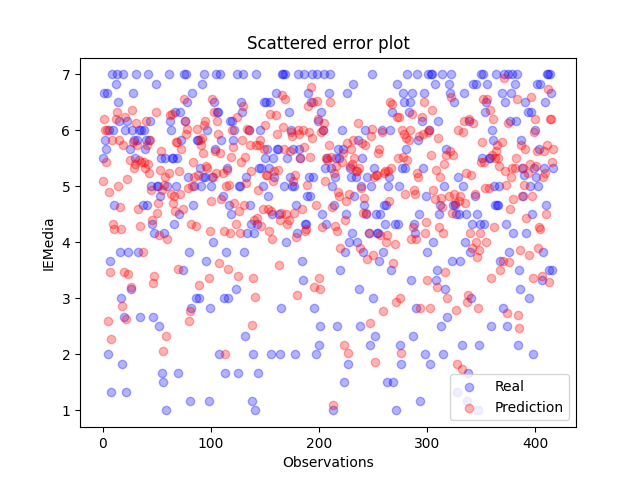
\includegraphics[scale=0.6]{scattered.png}
	\caption{Ejemplo de gráfico de dispersión de errores}
	\label{fig:scattered_example}
\end{figure}

El segundo gráfico consiste en lo siguiente:
Los modelos que han sido entrenados están prediciendo valores medios. El proceso seguido para realizar estos gráficos ha sido el de obtener los valores redondeados tanto de la predicción como del valor real. Si el valor redondeado de la predicción y del dato real son distintos, se ha considerado como error.  Sumando estos errores, se puede generar un gráfico de barras como el siguiente para tener una visión más clara de en que zonas de la predicción el algoritmo esta funcionando peor:
\linebreak
 \begin{figure}[H]
	\centering
	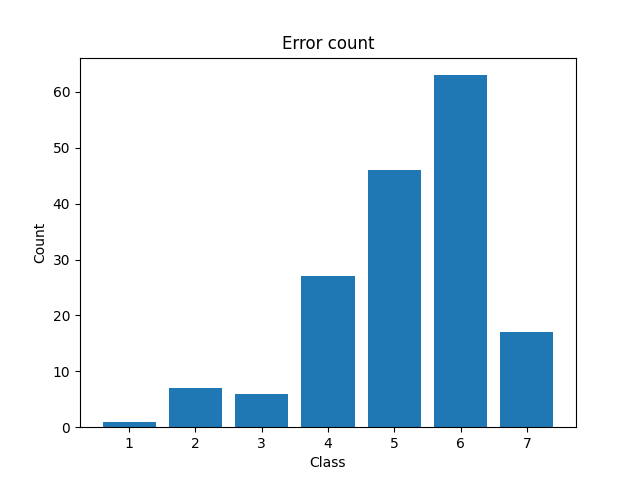
\includegraphics[scale=0.6]{error_hist.png}
	\caption{Ejemplo de gráfico de errores por rango}
	\label{fig:error_hist_example}
\end{figure}
\section{Modelos de regresión}
\subsection{Árboles de decisión}
\label{alg:dec_tree}
Los árboles de decisión son modelos que predicen la variable objetivo usando reglas del tipo \textit{si variable cumple condición entonces } inferidas a partir de los datos con los que se entrena el algoritmo.\\
Los árboles de decisión ofrecen ciertas ventajas:
\begin{enumerate}
	\item Son modelos fáciles de interpretar y pueden ser visualizados.
	\item Son capaces de trabajar con variables categóricas y numéricas.
	\item introducir alguna ventaja más
\end{enumerate}
Sin embargo, también presentan ciertas desventajas:
\begin{enumerate}
	\item Modelos que tienden al sobre-aprendizaje.
	\item No soportan valores perdidos.
	\item No trabajan bien con conjuntos de datos des-balanceados.
\end{enumerate}
Se ha seleccionado este modelo debido a que puede proporcionar información extra sobre conjunto de datos como la importancia de variables, que puede ser interesante a la hora de hacer uso de la información obtenida por los modelos.
\subsubsection*{Procesado de datos}
Antes de ejecutar la fase de entrenamiento, hay que modificar los datos para adaptarlos a las limitaciones del modelo. En este caso,  los Árboles de Decisión no admiten valores perdidos y debido a ciertas limitaciones de la librería que se está usando,  no son capaces de trabajar con variables categóricas, aunque generalmente si son capaces de trabajar con este tipo de variables..\\
Las modificaciones que se han hecho previamente son: (por orden)
\begin{enumerate}
	\item \textbf{Imputación de valores perdidos}
	\item \textbf{Transformación de variables categóricas a numéricas}
\end{enumerate}
 Por este motivo, se ha tenido que introducir una fase extra transformando las variables categóricas en numéricas.
\subsubsection*{Resultados}
\label{sec:res_tree}
Antes de mostrar los resultados, hay que destacar que cuando se entrena un árbol de decisión sin limitar los parámetros, este va a seguir separando los datos de entrenamiento hasta que no pueda realizar más divisiones. Para encontrar el árbol óptimo, primero se ha entrenado el árbol por defecto y se han obtenido los parámetros. Esos parámetros se han establecido como limite, se han entrenado varios árboles con distintos parámetros (sin superar el límite establecido por el primer modelo) y se ha escogido el que mejores resultados obtenía. Los parámetros que mejor resultados dieron son: \\
\begin{itemize}
	\item \textbf{Profundidad máxima:} Limita la profundidad (cantidad de preguntas) del árbol. El mejor valor ha sido \textbf{8}
	\item \textbf{Máximo número de hojas:} Máximo numero de hojas (grupos en el último nivel de una rama). El mejor valor ha sido \textbf{16}
\end{itemize}
En esta sección se va a exponer los resultados obtenidos usando  \textbf{Árboles de Decisión}.\\
La siguiente tabla expone los resultados obtenidos en validación:
\begin{table}[htbp]
    \centering
    \begin{tabular}{|c|c|c|c|c}
    \cline{1-4}
    Métricas         & R2    & Poisson deviance & MSE   \\ \cline{1-4}
    FOLD 1           & 0.678 & 0.211            & 0.886 \\ \cline{1-4}
    FOLD 2           & 0.65  & 0.213            & 0.913 \\ \cline{1-4}
    FOLD 3           & 0.629 & 0.239            & 0.98  \\ \cline{1-4}
    FOLD 4           & 0.679 & 0.187            & 0.779 \\ \cline{1-4}
    FOLD 5           & 0.636 & 0.211            & 0.933 \\ \cline{1-4}
    Media Validación & 0.654 & 0.212            & 0.898 \\ \cline{1-4}
    Test             & 0.69  & 0.196            & 0.815 \\ \cline{1-4}
    \end{tabular}
	\caption{Árbol de decisión:  Profundidad 8, número máximo de hojas 16}
	\label{tab:tree_res}
\end{table}
La siguiente figura muestra el gráfico de dispersión de errores:\\
 \begin{figure}[H]
	\centering
	\includegraphics[scale=0.8]{src/scattered_error_dtree.png}
	\caption{Gráfico de dispersión de errores}
	\label{fig:tree_scattered}
\end{figure}
Continuando con las gráficas, e continuación se muestra una gráfica con el conteo de errores por clase:
 \begin{figure}[H]
	\centering
	\includegraphics[scale=0.8]{src/error_hist_dtree.png}
	\caption{Conteo de errores}
	\label{fig:tree_error_plot}
\end{figure}
\subsubsection*{Representación}
Como se mencionó en la sección \textbf{\ref{alg:dec_tree}-\nameref{alg:dec_tree}}, los árboles de decisión tienen la ventaja de que pueden representarse fácilmente. \\
En este caso, vamos a usar una representación gráfica del árbol, las reglas que ha obtenido el árbol y las variables más importantes.\\
\linebreak
La siguiente figura muestra la representación gráfica del árbol de decisión entrenado:\\
\linebreak
 \begin{figure}[H]
	\centering
	\includegraphics[scale=0.2]{src/dtree_plot.png}
	\caption{Árbol de decisión}
	\label{fig:decission_tree1}
\end{figure}
A continuación se muestra en pseudo-código, las reglas que ha inferido el árbol de decisión:\\

\begin{figure}[H]
	\begin{lstlisting}
def predict(sample):
	if AE5 <= 4.5:
		if AcMedia <= 3.1:
			if AE5 <= 1.5:
				return 1.28
			else:  # if AE5 > 1.5
				return 2.12
		else:  # if AcMedia > 3.1
			if SE2 <= 3.5:
				if BA3.f <= 0.5:
					return 3.27
				else:  # if BA3.f > 0.5
					return 4.61
			else:  # if SE2 > 3.5
				if Beca <= 0.75:
					if Nota <= 6.85:
						return 3.46
					else:  # if Nota > 6.85
						return 4.52
				else:  # if Beca > 0.75
					return 3.32
	else:  # if AE5 > 4.5
		if AE5 <= 5.75:
			if SE2 <= 3.5:
				if CEF19 <= 3.75:
					return 4.7
				else:  # if CEF19 > 3.75
					return 3.79
			else:  # if SE2 > 3.5
				return 5.19
		else:  # if AE5 > 5.75
			if AcMedia <= 6.55:
				if SE5 <= 1.5:
					return 2.75
				else:  # if SE5 > 1.5
					if NS1 <= 6.75:
						return 5.5
					else:  # if NS1 > 6.75
						if AE7 <= 2.75:
							return 4.69
						else:  # if AE7 > 2.75
							return 6.13
			else:  # if AcMedia > 6.55
				if SEMedia <= 3.58:
					return 5.68
				else:  # if SEMedia > 3.58
					return 6.6
	\end{lstlisting}
\caption{Reglas del árbol de decisión}
\label{fig:tree_rules}
\end{figure}
\pagebreak
Por ultimo, estas son las 10 variables que el modelo consideró con más relevancia. El valor asociado a cada variable es la \textbf{importancia Gini}:
\begin{figure}[H]
	\centering
	\includegraphics[scale=0.25]{src/feature_importance_dtree}
	\caption{10 variables más importantes segun AD}
	\label{fig:feature_dtree}
\end{figure}
Volviendo a la documentación proporcionada para comprobar el significado de esos valores:
\begin{itemize}
	\item \textbf{AE5:} Pregunta  5 sobre Actitudes financieras empresariales. Valor $0.735667$
	\item \textbf{AcMedia:} Variable global de Actitud emprendedora. Valor $0.156046$
	\item \textbf{SE2:} Estoy preparado para iniciar una empresa viable. Valor $0.037300$
	\item \textbf{SE5:} Conozco cómo desarrollar un proyecto empresarial. Valor $0.014692$
	\item \textbf{NS1:} Mi familia aprobaría el que yo decidiese crear una empresa. Valor $0.012393$
	\item \textbf{Beca:} Tiene beca el encuestado. Valor $0.008256$
	\item \textbf{Nota:} Nota media del expediente académico hasta la fecha de la encuesta sobre 10 puntos. Valor $0.008034$
	\item \textbf{BA3.f:} En los últimos 12 meses, ¿has ahorrado personalmente algún dinero de alguna de las siguientes formas, independientemente de si aún dispones del dinero? Han contestado las opciones a, c, d, e, f, g (en casa, en cuenta de ahorro, darlo a la familia, productos de inversión, de otro modo). Valor $0.007389$
	\item \textbf{CEF19:} Pregunta sobre Conocimientos financieros empresariales. Valor $0.007202$
	\item \textbf{AE7:} Pregunta 7 sobre Actitudes financieras empresariales. Valor $0.006518$
\end{itemize}
De las columnas \textit{AEx} y \textit{CEFx} no hay información en la documentación, unicamente se menciona que son una serie de preguntas relacionadas con actitudes financieras empresariales y sobre conocimientos financieros empresariales respectivamente.
\subsection{Random Forest}
\label{sec:rf}
Random Forest es un modelo  combinado de aprendizaje que puede usarse para clasificación y/o regresión. Random Forest consiste en un conjunto de árboles de decisión que operan juntos. Una vez que cada árbol dentro del Random Forest realiza una predicción, se escoge la predicción con más votos. \\ Se ha escogido este modelo ya que como se comprobó en la sección \textbf{\ref{alg:dec_tree}-\nameref{alg:dec_tree}}, los árboles de decisión dieron buenos resultados
\linebreak
Para que Random Forest funciona bien, hay que asegurar que los distintos árboles que lo forman tengan una baja \textbf{correlación} entre ellos. Esto quiere decir que los árboles tienen que diferir y proporcionar predicciones distintas, de esta manera, si hay un conjunto de  árboles que da una predicción malas, puede haber otro conjunto que vaya en la dirección correcta. \\
\linebreak
Los Árboles de Decisión son modelos que son muy sensibles a los datos con los que se ha entrenado, por lo que cualquier cambio en los datos de entrenamiento puede hacer que cambie una predicción. Random Forest hace uso de esta peculiaridad de los árboles de decisión.
En el momento de entrenar los distintos árboles, en vez de usar subconjuntos del conjunto de entrenamiento se usan $N$ conjuntos del mismo tamaño que el conjunto de entrenamiento obtenidos usando un \textbf{muestreo con reemplazo}. Una vez que se tienen los distintos conjuntos, se entrena cada conjunto con un árbol. Este proceso se conoce como \textbf{bagging}.\\
\linebreak
Una peculiaridad más que tiene Random Forest es la forma con la que los árboles seleccionan la variable que van a usar para dividir el conjunto de datos. Estos no eligen la variable en función de un criterio concreto, si no que eligen la variable usando un conjunto aleatorio de las características.  Esto fuerza a que los árboles sean mas diferentes entre ellos, bajando la correlación entre los árboles que forman el modelo.
\subsubsection*{Procesado de datos}
Al igual que los árboles de decisión, se ha hecho una imputación de valores perdidos y se ha transformado las variables categóricas a numéricas debido a limitación que hay en la librería usada.
\pagebreak
\subsubsection*{Resultados}
Antes de mostrar los resultados, estos son los parámetros que se han usado al entrenar el modelo:
\begin{itemize}
	\item \textbf{max\_features}:  Número de variables que se van a escoger de manera aleatoria: $\frac{1}{3}$ del número de variables.
	\item\textbf{n\_estimators}: Número de árboles que forman el Random Forest: $500$
\end{itemize}
En la siguiente tabla, se muestra el resultado para obtenidos en validación y en test:
\linebreak
\begin{table}[H]
	\centering
	\begin{tabular}{|c|c|c|c|c}
		\cline{1-4}
		Métricas          & R2    & Poisson deviance & MSE   \\ \cline{1-4}
		FOLD 1            & 0.765 & 0.156            & 0.647 \\ \cline{1-4}
		FOLD 2            & 0.778 & 0.136            & 0.577 \\ \cline{1-4}
		FOLD 3            & 0.735 & 0.174            & 0.7   \\ \cline{1-4}
		FOLD 4            & 0.732 & 0.152            & 0.65  \\ \cline{1-4}
		FOLD 5            & 0.751 & 0.147            & 0.639 \\ \cline{1-4}
		Media  Validación & 0.752 & 0.153            & 0.643 \\ \cline{1-4}
		Test     		  & 0.768  & 0.15            & 0.609 \\ \cline{1-4}
	\end{tabular}
	\caption{Random Forest}
	\label{tab:res_random_forest}
\end{table}
La siguiente figura muestra el gráfico de dispersión de errores:\\
\linebreak
\begin{figure}[H]
	\centering
	\includegraphics[scale=0.7]{src/scattered_error_rf.png}
	\caption{Gráfico de dispersión de errores}
	\label{fig:rf_scattered}
\end{figure}
Continuando con las gráficas, e continuación se muestra una gráfica con el conteo de errores por clase:
\begin{figure}[H]
	\centering
	\includegraphics[scale=0.7]{src/error_hist_rf.png}
	\caption{Conteo de errores}
	\label{fig:rf_error_plot}
\end{figure}
Para finalizar, esta es la lista de las 10 variables más importantes que ha obtenido Random Forest:
\begin{figure}[H]
	\centering
	\includegraphics[scale=0.6]{src/feature_importance_rf}
	\caption{10 variables más importantes según RF}
	\label{fig:feature_rf}
\end{figure}
Volviendo a la documentación, esta es la explicación para cada variable:
\begin{itemize}
	\item\textbf{AE5:} Pregunta  5 sobre Actitudes financieras empresariales. Valor = $0.246364$
	\item\textbf{AcMedia:} Variable global de Actitud emprendedora. Valor = $0.220202$
	\item\textbf{AC2:} Ser emprendedor es una salida profesional atractiva para mí. Valor = $0.072907$
	\item\textbf{AC4:}Ser emprendedor supondría una gran satisfacción para mí. Valor = $0.065776$
	\item\textbf{AC3:} Si tuviera la oportunidad y los recursos, me gustaría iniciar una empresa. Valor = $0.041642$
	\item\textbf{SEMedia:} Variable global de Autoeficacia emprendedora. Valor = $0.022872$
	\item\textbf{SE2:} Estoy preparado para iniciar una empresa viable. Valor = $0.019630$
	\item\textbf{AC1:} Ser emprendedor implica más ventajas que desventajas para mí. Valor = $0.019396$
	\item\textbf{NS1:} Mi familia aprobaría el que yo decidiese crear una empresa. Valor = $0.014467$
	\item\textbf{Nota:} Nota media del expediente académico hasta la fecha de la encuesta sobre 10 puntos. Valor = $0.012254$
\end{itemize}
\subsection{KNN}
\label{alg:knn}
KNN (\textit{K Nearest Neighbors}) es un algoritmo supervisado basado en instancias. Este algoritmo no aprende un modelo si no que almacena todas las muestras de entrenamiento y cuando hay que predecir una nueva ejemplo, el algoritmo usa las muestras almacenadas calculando la distancia a cada muestra y obteniendo los K vecinos más cercanos y usando las valores reales de los vecinos seleccionados, asigna una predicción al ejemplo a predecir, generalmente asignando aquella clase con más "votos".\\
\linebreak
Para medir la distancia entre dos muestras, KNN puede usar una gran cantidad métricas, las más comunes son:
\begin{itemize}
	\item \textbf{Distancia euclidiana:} Definida como $\sqrt{\sum(x_1 - x_2)^2}$
	\item \textbf{Distancia Manhattan:} Definida como $\sum|x_1 - x_2|$
	\item \textbf{Distancia Minkowski:} Definida como $(\sum|x_1 - x_2|^p)^{\frac{1}{p}}$, siendo P un entero positivo
\end{itemize}
La implementación del algoritmo KNN de ScikitLearn usa por defecto la distancia \textbf{Minkowski}. Esta tiene la peculiaridad de que cambiando el parámetro $p$ puede usarse la distancia euclidiana ($p=2$) o la distancia Manhattan ($p=1$)
\subsubsection*{Procesado de datos}
KNN es un algoritmo que depende de la distancia entre dos muestras, esto implica que si una caracteristica del conjunto de datos que se esta usando tiene un rango \textbf{mayor} que otra, esa característica aportará más al cálculo de la distancia, cuando no necesariamente debe de ser así. Por ese motivo, este algoritmo necesita que el conjunto de datos esté \textbf{normalizado} en el momento de entrenar.\\
\linebreak
Este algoritmo, a parte de necesitar que los datos estén normalizados, no admite valores perdidos y variables categóricas.

\subsubsection*{Resultados}
Antes de mostrar los resultados, estos son los parámetros que se han usado al entrenar el algoritmo:
\begin{itemize}
	\item \textbf{K:} Número de vecinos: 5
	\item \textbf{Métrica:} Distancia usada: Minkowski con $P=2$ (distancia euclidiana).
\end{itemize}
En la siguiente tabla, se muestra el resultado para obtenidos en validación y en test:
\linebreak
\begin{table}[H]
	 \centering
	\begin{tabular}{|c|c|c|c|c}
		\cline{1-4}
		Métricas         & R2    & Poisson deviance & MSE   \\ \cline{1-4}
		FOLD 1           & 0.47  & 0.356            & 1.46  \\ \cline{1-4}
		FOLD 2           & 0.407 & 0.378            & 1.545 \\ \cline{1-4}
		FOLD 3           & 0.449 & 0.362            & 1.457 \\ \cline{1-4}
		FOLD 4           & 0.435 & 0.329            & 1.372 \\ \cline{1-4}
		FOLD 5           & 0.467 & 0.321            & 1.367 \\ \cline{1-4}
		Media Validación & 0.446 & 0.349            & 1.44  \\ \cline{1-4}
		Test             & 0.527 & 0.301            & 1.242 \\ \cline{1-4}
	\end{tabular}
	\caption{KNN: $K=5$, métrica Minkowski con $P=2$}
	\label{tab:knn_res}
\end{table}
La siguiente figura muestra el gráfico de dispersión de errores:
\begin{figure}[H]
	\centering
	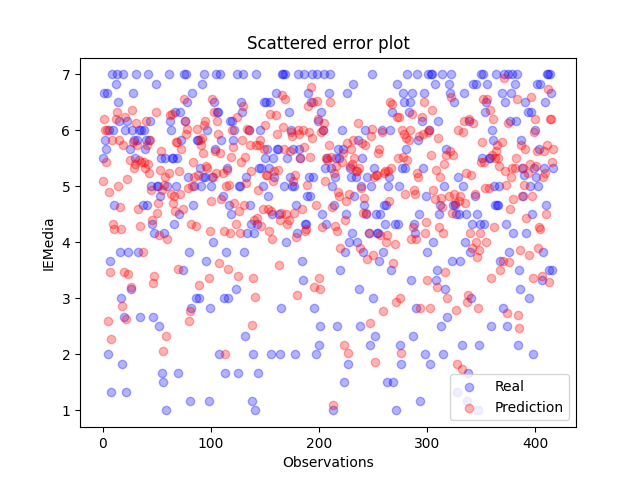
\includegraphics[scale=0.8]{src/scattered_error_knn.png}
	\caption{Gráfico de dispersión de errores}
	\label{fig:knn_scattered}
\end{figure}
Continuando con las gráficas, e continuación se muestra una gráfica con el conteo de errores por clase:\\
\linebreak
\begin{figure}[H]
	\centering
	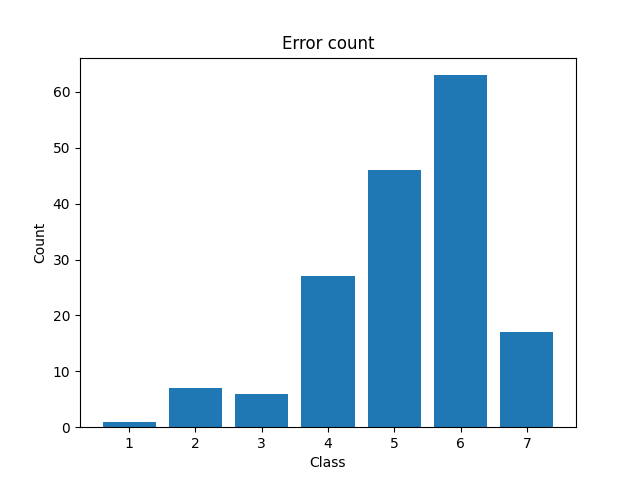
\includegraphics[scale=0.8]{src/error_hist_knn.png}
	\caption{Conteo de errores}
	\label{fig:knn_error_plot}
\end{figure}
\subsection{SVM}
\label{sec:svm}
Maquina de soporte de vectores (Support Vector Machines) es un modelo de aprendizaje supervisado cuyo objetivo es encontrar un hiper-plano dentro de un espacio de  $N$ dimensiones ($N$ es el número de características del conjunto de datos) que clasifique las muestras de dentro del espacio en distintas clases.  Originalmente, se diseñó para clasificación binaria, pero en la actualidad este algoritmo se ha adaptado para regresión, clasificación multi-clase y  multi-etiqueta\\
\linebreak
Pueden existir muchos hiper-planos que separen los puntos del espacios en distintas clases. El objetivo de SVM es encontrar aquel hiper-plano con mayor \textbf{margen} (distancia entre puntos de distintas clases),  ya que incrementa la posibilidad de clasificar correctamente muestras que no se han usado en entrenamiento al disponer de un margen mayor de error. Los vectores soporte son aquellas observaciones del conjunto de datos que definen el hiper-plano. Idealmente, estas o\\
\begin{figure}[H]
	\centering
	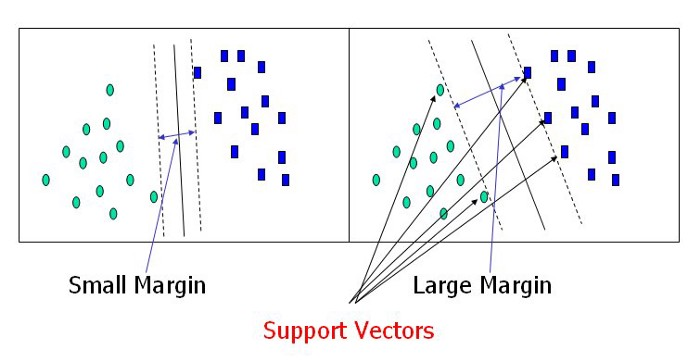
\includegraphics[scale=0.5]{svm}
	\caption{Ejemplo de SVM en dos dimensiones}
	\label{fig:svm}
\end{figure}
\subsubsection*{Procesado de datos}
SVM son modelos con una fuerte base matemática, por lo que son modelos que no pueden ser entrenados usando variables categóricas.
Las modificaciones que se han hecho previamente son: (por orden)
\begin{enumerate}
	\item \textbf{Imputación de valores perdidos.}
	\item \textbf{Escalado de valores numéricos.}
	\item \textbf{Transformación de variables categóricas a numéricas.}
\end{enumerate}
\subsubsection*{Resultados}
A continuación se muestra una tabla con los resultados obtenidos por SVM en el conjunto de validación y en el conjunto de test:
\begin{table}[H]
	  \centering
	\begin{tabular}{|l|l|l|l|l}
		\cline{1-4}
		Métricas         & R2      & Poisson deviance & MSE   \\ \cline{1-4}
		FOLD 1   		 & 0.671   & 0.236            & 0.906 \\ \cline {1-4}
		FOLD 2   		 & 0.718   & 0.186            & 0.734 \\ \cline {1-4}
		FOLD 3   		 & 0.728   & 0.185            & 0.72  \\ \cline {1-4}
		FOLD 4   		 & 0.691   & 0.192            & 0.75  \\ \cline {1-4}
		FOLD 5   		 & 0.697   & 0.193            & 0.776 \\ \cline {1-4}
		Media Validación & 0.701   & 0.198            & 0.777 \\ \cline {1-4}
		Test             & 0.737   & 0.173            & 0.691 \\ \cline {1-4}
	\end{tabular}
\caption{SVM: Tolerancia $1^{-3}$, Kernel RBF, $C=1$}
\label{tab:svm_res}
\end{table}
La siguiente figura muestra el gráfico de dispersión de errores:
\begin{figure}[H]
	\centering
	\includegraphics[scale=0.8]{src/scattered_error_svr.png}
	\caption{Gráfico de dispersión de errores}
	\label{fig:svr_scattered}
\end{figure}
Continuando con las gráficas, e continuación se muestra una gráfica con el conteo de errores por clase:\\
\linebreak
\begin{figure}[H]
	\centering
	\includegraphics[scale=0.8]{src/error_hist_svr.png}
	\caption{Conteo de errores}
	\label{fig:svr_error_plot}
\end{figure}
\subsection{XGBoost}
Extreme Gradient Boosting  es un método de aprendizaje combinado basado en árboles de decisión.\\
A diferencia de Random Forest (que también es un método combinado basado en árboles de decisión), XGBoost hace uso de técnicas de \textit{Gradient Boosting}  frente a Random Forest que hace uso de \textit{Bagging} para entrenar los modelos que lo forman. (\ref{sec:rf}-\nameref{sec:rf}).\\
\linebreak
\textit{Boosting} se basa en la unión de varios modelos débiles para formar un modelo que en conjunto. Estos modelos débiles se van entrenando de forma iterativa, adaptando los parámetros del modelo en cada iteración,  teniendo en cuenta que estos modelos no deben aumentar en complejidad y deben mantener un rendimiento mínimo (idealmente, mejor que un clasificador aleatorio).\\
\linebreak
\textit{Grandient Boosting} es un caso especial de \textit{Boosting} en el que se hace uso del algoritmo  \textbf{Gradiente Descendente} para minimizar los errores de los modelos simples.\\
\linebreak
Finalmente, XGBoost funciona añadiendo secuencialmente Árboles de Decisión, de tal manera que cada árbol reduzca el error de los previos aprendiendo de los errores que han cometido los árboles anteriores. 
\subsubsection*{Procesado de datos}
El pre-procesado aplicado para este modelo ha sido similar al usado en Árboles de Decisión:
\begin{enumerate}
	\item \textbf{Imputación de valores perdidos}
	\item \textbf{Transformación de variables categóricas a numéricas}
\end{enumerate}
\subsubsection*{Resultados}
A continuación se muestra una tabla con los resultados obtenidos por \textbf{XGBoost} en los conjuntos de validación, train y test:
\begin{table}[H]
	 \centering
	\begin{tabular}{|c|c|c|c|c|}
		\cline{1-4}
		Métricas         &	 R2  & Poisson deviance & MSE   \\ \cline{1-4}
		FOLD 1           & 0.724 & 0.188            & 0.759 \\ \cline{1-4}
		FOLD 2           & 0.73  & 0.166            & 0.704 \\ \cline{1-4}
		FOLD 3           & 0.712 & 0.195            & 0.761 \\ \cline{1-4}
		FOLD 4           & 0.72  & 0.162            & 0.679 \\ \cline{1-4}
		FOLD 5           & 0.744 & 0.156            & 0.658 \\ \cline{1-4}
		Media Validación & 0.726 & 0.173            & 0.712 \\ \cline{1-4}
		Test             & 0.74  & 0.163            & 0.682 \\ \cline{1-4}
	\end{tabular}
		\caption{Métricas de XGBoost con}
		\label{tab:xgboost}
\end{table}
La siguiente figura muestra el gráfico de dispersión de errores:
\begin{figure}[H]
	\centering
	\includegraphics[scale=0.8]{src/scattered_error_xgboost.png}
	\caption{Gráfico de dispersión de errores para XGBoost}
	\label{fig:xgboost_scattered}
\end{figure}
Finalizando con las gráficas, a continuación se muestra una gráfica con el conteo de errores por clase:
\begin{figure}[H]
	\centering
	\includegraphics[scale=0.8]{src/error_hist_xgboost.png}
	\caption{Conteo de errores}
	\label{fig:xgboost_error_plot}
\end{figure}

\subsection{Perceptrón multicapa}
El Perceptrón Multicapa es un modelo de aprendizaje supervisado basada en red neuronales artificiales y haciendo uso del algoritmo \textbf{Perceptrón}.\\
\linebreak
El Perceptrón es un algoritmo de aprendizaje supervisado para clasificación binaria. Es un clasificador linear que funciona iterando sobre cada muestra del conjunto de datos hasta calcular un hiper-plano que separe el conjunto de datos. Los pasos de este algoritmo son: 
\begin{enumerate}
	\item Establecer un plano inicial (generalmente de manera aleatoria ).
	\item Por cada muestra del conjunto de datos, si la muestra está mal clasificada, se modifican los pesos que definen el hiper-plano para clasificar correctamente esa muestra.	
	\item El paso anterior se repite hasta que todas las muestras estén bien clasificadas ó no se haya hecho ninguna modificación. Por lo general, también se añade un número máximo de iteraciones que se van a realizar.
\end{enumerate}
Este algoritmo tiene una limitación muy fuerte: No puede resolver problemas no lineales (incluso funciones sencillas como la \textit{XOR}). \\
\linebreak
Para afrontar este problema, se propuso el usar una combinación de perceptrones siguiendo una estructura de red neuronal, consiguiendo así un modelo capaz de resolver problemas no lineales. Estas redes neuronales tienen al menos 3 capas:
\begin{itemize}
	\item Capa de entrada: Está formada por las primeras neuronas que forman la red y se encargan de introducir los datos a la red.
	\item Capa/s oculta: Son las capas de la zona media de la red y son las encargadas del procesamiento de los datos para formar el modelo.
	\item Capa de salida: Dan el valor de salida del modelo.
\end{itemize}
\begin{figure}[H] 
	\centering
	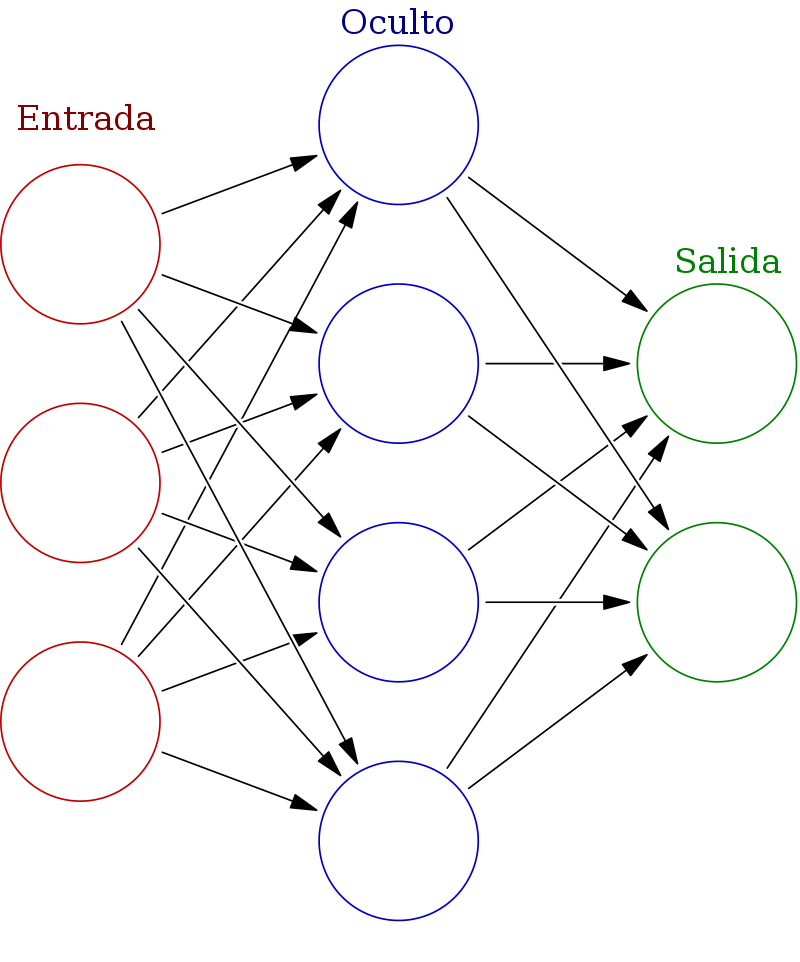
\includegraphics[scale=0.3]{rnn}
	\caption{Ejemplo de Red Neuronal con 1 capa oculta}
	\label{fig:rnn}
\end{figure}
Un elemento fundamental de las Redes Neuronales es el algoritmo de \textit{back-propagation}. Este algoritmo usa el error obtenido en las capas de salida y este era propagado hacia cada neurona anterior (de ahí el nombre de \textit{back-propagation}), ajustando así el peso calculado por cada neurona en función del comportamiento del modelo en la iteración anterior.
\subsubsection*{Procesado de datos}
Como se puede apreciar, el MLP son algoritmos con una fuerte base matemática, por lo que no son capaces de ser entrenados usando variables categóricas. Las modificaciones que se han hecho sobre el conjunto de datos son las siguientes:
\begin{enumerate}
	\item \textbf{Imputación de valores perdidos.}
	\item \textbf{Escalado de valores numéricos.}
	\item \textbf{Transformación de variables categóricas a numéricas.}
\end{enumerate}
\subsubsection*{Resultados}
En esta sección se va a mostrar los resultados obtenidos por el Perceptrón Multi-capa. \\
\linebreak
En esta tabla, se puede observar el rendimiento del modelo en los conjuntos de validación, entrenamiento y test:
\begin{table}[H]
	\centering
	\begin{tabular}{|c|c|c|c|c}
		\cline{1-4}
		Métricas         & R2    & Poisson deviance & MSE   \\ \cline{1-4}
		FOLD 1           & 0.569 & 0.275            & 1.187 \\ \cline{1-4}
		FOLD 2           & 0.652 & 0.23             & 0.907 \\ \cline{1-4}
		FOLD 3           & 0.609 & 0.255            & 1.033 \\ \cline{1-4}
		FOLD 4           & 0.401 & 0.279            & 1.454 \\ \cline{1-4}
		FOLD 5           & 0.567 & 0.251            & 1.112 \\ \cline{1-4}
		Media Validación & 0.56  & 0.258            & 1.139 \\ \cline{1-4}
		Test	         & 0.625 & 0.244            & 0.984 \\ \cline{1-4}
	\end{tabular}
	\caption{Perceptrón Multicapa: 2 capas de 100 neuronas, 500 iteraciones}
	\label{tab:mlp_res}
\end{table}
La siguiente figura muestra el gráfico de dispersión de errores:
\begin{figure}[H]
	\centering
	\includegraphics[scale=0.8]{src/scattered_error_MLP.png}
	\caption{Gráfico de dispersión de errores}
	\label{fig:mlp_scattered}
\end{figure}
Continuando con las gráficas, e continuación se muestra una gráfica con el conteo de errores por clase:\\
\linebreak
\begin{figure}[H]
	\centering	\includegraphics[scale=0.8]{src/error_hist_MLP.png}
	\caption{Conteo de errores}
	\label{fig:mlp_error_plot}
\end{figure}
\section{Conclusiones}
Se ha observado que los modelos basados en Árboles de Decisión y Random Forest han tenido un buen comportamiento, por lo que se ha optado por seguir haciendo uso de ellos en secciones siguientes. XGBoost, tiene unos resultados ligeramente peores respecto a Random Forest pero con un comportamiento similar, fallando considerable en valores altos de intención emprendedora media). Como XGBoost no esta aportando nada nuevo, por ahora se va a descartar.\\
\linebreak
SVR se ha comportado casi al nivel de modelos como XGBoost o Random Forest. Por ahora, no se va a descartar su uso, ya que introduciendo el conocimiento que se ha obtenido usando modelos como Random Forest o árboles de decisión se podría mejorar el rendimiento.\\
\linebreak
Los resultados obtenidos por  KNN demuestran que este algoritmo no funciona bien con el conjunto de datos que se está usando. La razón más probable por la que KNN obtuvo estos resultados, es que hay relaciones entre las variables que KNN no es capaz de detectar, al comparar únicamente la distancia característica por característica. Debido al bajo desempeño que se ha obtenido al usar KNN, va a ser descartado de las siguientes fases.\\
\linebreak
Respecto al Perceptrón Multicapa, ya que el rendimiento en comparación con otros modelos probados y debido al enorme coste de entrenamiento que pueden llegar a tener, se ha decidido no continuar haciendo uso de este modelo.\\
\linebreak
Como ya se ha mencionado, los modelos basados en árboles de decisión son capaces de obtener la importancia de las características. A continuación se muestran las gráficas de nuevo para facilitar la comparación:
\begin{figure}[H]
	\centering
	\includegraphics[scale=0.5]{src/feature_importance_dtree}
	\caption{10 variables más importantes según árboles de decisión}
	\label{fig:feature_dtree2}
\end{figure}
\begin{figure}[H]
	\centering
	\includegraphics[scale=0.5]{src/feature_importance_rf}
	\caption{10 variables más importantes según RF}
	\label{fig:feature_rf2}
\end{figure}
Como se ve en las figuras, vemos que hay dos variables que \textbf{ambos} algoritmos han dado como más importantes:
\begin{itemize}
	\item\textbf{AE5:} Pregunta  5 sobre Actitudes financieras empresariales.
	\item\textbf{AcMedia:} Variable global de Actitud emprendedora.
\end{itemize}
Repasando los resultados, se puede apreciar que a todos los algoritmos usados les está costando predecir correctamente los valores altos para la intención emprendedora media (véase figura \ref{fig:rf_error_plot}). Este comportamiento ha sido constante para cada algoritmo usado. La causa de este comportamiento puede ser que a medida que se incrementa el valor de intención emprendedora media, los datos son menos dispersos y a los algoritmos les está costando distinguir entre varios valores cercanos. Este comportamiento se puede apreciar en los gráficos de dispersión de errores que se han mostrado previamente.
 \pagebreak
\section{Muestreo de datos}
Una vez se ha comprobado el rendimiento de los distintos modelos que se han seleccionado, se va a intentar mejorarlo añadiendo nuevas etapas extra al procesamiento de datos antes de entrenar los modelos.
\newline
Como se ha podido observar en la primera iteración, todos los algoritmos se están equivocando en valores altos. Para intentar reducir el ruido, se va tratar el conjunto de datos haciendo \textbf{under-sampling}.\\
Under-Sampling (se podría traducir como \textit{muestreo}) es una técnica para reducir el ruido del conjunto de datos eliminando algunas muestras del conjunto de datos.\\
\linebreak
Como se puede ver en la \ref{tab:ocurrencia_valores} donde se muestra la ocurrencia de valores para las distintas variables a predecir,  aquellos con un valor alto son los más predominantes, siendo en estos valores donde los algoritmos más se están equivocando. El motivo puede ser que al estar prediciendo la media de las distintas variables, se está introduciendo una gran cantidad de ruido. \\
En valores bajos, como se puede ver en la figura \ref{fig:rf_error_plot} donde se muestra el gráfico de errores para Random Forest, la cantidad de fallos en el algoritmo para estos valores es mucho menor. Esta tendencia se repite en todos los algoritmos.\\
\subsection{Algoritmo}
 Para realizar el proceso de muestreo, se ha desarrollado el siguiente algoritmo:
 \begin{enumerate}
 	\item Se entrena un modelo de aprendizaje con el conjunto de entrenamiento.
 	 \item Por cada muestra del conjunto de entrenamiento, se predice el valor usando el modelo entrenado.
 	 \item Se comprueba la diferencia entre valor real y el valor predicho.
 	 \item Si la diferencia es mayor que un umbral, se elimina esa muestra del conjunto de entrenamiento.
 \end{enumerate}
La función que ejecuta este simple algoritmo de muestreo se llama \textit{\textbf{regression\_under\_sampler}}.
\linebreak
El modelo entrenado para hacer muestreo, es un árbol de decisión con un máximo de $4$ niveles, eliminando muestras de todo el rango de predicción.
 \subsection{Resultados}
 A continuación se muestra una serie de gráficos comparando los resultados obtenidos por los algoritmos seleccionados:
 \subsubsection*{Árboles de Decisión}
\begin{figure}[H]
	\centering
	\includegraphics[scale=0.8]{src/dtree_undersamp_error_hist.png }
	\caption{Comparación de errores usando under-sampling}
	\label{fig:cmp_error_dtree}
\end{figure}
Como se aprecia en la figura \ref{fig:cmp_error_dtree}, usando el algoritmo de muestreo, se ha reducido la cantidad ruido en los rangos más altos de predicción, mejorando así el rendimiento del árbol de decisión para estos valores y estabilizando las zonas donde se estaba comportando peor.
\begin{figure}[H]
	\centering
	\includegraphics[scale=0.8]{src/dtree_undersamp_val_metrics.png}
	\caption{Media en validación usando under-sampling}
	\label{fig:cmp_val_dtree}
\end{figure}
Esta gráfica compara el rendimiento medio en el conjunto de validación.
Respecto a las métricas obtenidas en los conjuntos de validación, se puede apreciar que en cuanto al valor obtenido por $R2$ se ha mantenido, pero se ha mejorado drásticamente el valor en las métricas \textit{Desviación de Poisson} y \textit{MSE}. Esto indica que el modelo obtenido tras el procesamiento se ajusta mejor a los datos.
\begin{figure}[H]
	\centering
	\includegraphics[scale=0.8]{src/dtree_undersamp_test_metrics.png}
	\caption{Métricas en test usando under-sampling}
	\label{fig:cmp_test_dtree}
\end{figure}
Como se puede ver en la imagen anterior, las métricas en test son ligeramente mejores tras reducir el ruido dentro del conjunto de entrenamiento.\\
\linebreak
En general, se aprecia una mejora en árboles de decisión reduciendo el ruido del conjunto de datos, ya que los árboles de decisión son algoritmos bastantes sensibles al ruido.
\subsubsection*{SVR}
\begin{figure}[H]
	\centering
	\includegraphics[scale=0.8]{src/svr_undersamp_error_hist.png }
	\caption{Comparación de errores usando under-sampling}
	\label{fig:cmp_error_svr}
\end{figure}
Al contrario que los Árboles de Decisión, SVM han sido menos propicias al ruido del conjunto de datos. Al aplicar el muestreo se aprecia una bajada de rendimiento en todos los rangos de predicción. \\
Como se explicaba en \nameref{sec:svm} - \ref{sec:svm}, SVM busca el hiperplano con más margen entre los clusters que forma el conjunto de datos, consiguiendo así un algoritmo robusto frente a ruido. 
\begin{figure}[H]
	\centering
	\includegraphics[scale=0.8]{src/svr_undersamp_val_metrics.png}
	\caption{Media en validación usando under-sampling}
	\label{fig:cmp_val_svr}
\end{figure}
\begin{figure}[H]
	\centering
	\includegraphics[scale=0.8]{src/svr_undersamp_test_metrics.png}
	\caption{Métricas en test usando under-sampling}
	\label{fig:cmp_test_svr}
\end{figure}
Las gráficas \ref{fig:cmp_val_svr} y \ref{fig:cmp_test_svr} complementan el resultado mostrado en la gráfica \ref{fig:cmp_error_svr}, las cuales demuestran que la mejora apreciada en Árboles de Decisión no ha aplicó en SVM y lejos de mejorar, ha empeorado el valor obtenido por algunas métricas de regresión.\\ 
\subsubsection*{Random Forest}
\begin{figure}[H]
	\centering
	\includegraphics[scale=0.8]{src/rf_undersamp_error_hist.png }
	\caption{Comparación de errores usando under-sampling}
	\label{fig:cmp_error_rf}
\end{figure}
En la figura se puede apreciar como al igual que los Árboles de decisión, el eliminar ciertas instancias ruidosas del conjunto de datos implica una mejora en el rendimiento del algoritmo. En este caso, se ha conseguido reducir el porcentaje de fallos cuando se está prediciendo valores altos de intención emprendedora media.
\begin{figure}[H]
	\centering
	\includegraphics[scale=0.8]{src/rf_undersamp_val_metrics.png}
	\caption{Media en validación usando under-sampling}
	\label{fig:cmp_val_rf}
\end{figure}
En cuanto a la media en validación, a medida que se reduce la cantidad de muestras eliminadas, se aprecia como se reduce la métrica $R2$ pero mejora las métricas MSE y Desviación Poisson.
\begin{figure}[H]
	\centering
	\includegraphics[scale=0.8]{src/rf_undersamp_test_metrics.png}
	\caption{Métricas en test usando under-sampling}
	\label{fig:cmp_test_rf}
\end{figure}
En test se aprecia el mismo comportamiento que en los conjuntos de validación: el mejor valor para $R2$ ha sido el obtenido entrando el modelo sin aplicar el  muestreo, mientras que respecto al resto de métricas, ha obtenido los mejores resultados eliminando las muestras problemáticas.\\
\subsection{Conclusiones}
Se ha apreciado una mejora en en los algoritmos basados en árboles de decisión. La principal mejora ha sido el obtener una menor cantidad de errores en aquellas zonas donde los algoritmos se están comportando peor. También se ha podido observar que Random Forest obtuvo mejores resultados con un umbral más alto que Árboles de Decisión. \\
La causa más probable de que necesite un umbral más alto es que al usar varios árboles para predecir el resultado, la probabilidad de que varios árboles contradigan el valor predicho por un árbol que clasificó mal un valor es alta. Por eso, al eliminar aquellas muestras más problemáticas del conjunto, el propio Random Forest es capaz de lidiar con el ruido de muestras que son menos problemáticas y beneficiarse de tener un conjunto de entrenamiento más grande.\\
\linebreak
Respecto a SVM, observando los resultados obtenidos, se aprecia que ha medida que se reduce la cantidad de muestras que se eliminan, el rendimiento es mejor. 
Como se están eliminando muestras que pueden estar en la frontera (o incluso vectores soporte),, es posible que el hiper-plano calculado por el modelo de un menor margen o sea en general peor. 
	\pagebreak

	\chapter{Clasificación a partir de regresión}

Se ha comprobado que usando regresión, se ha conseguido unos buenos modelos para predecir un valor \textbf{preciso} de la intención emprendedora media. El siguiente paso realizado ha sido el de \textbf{categorizar} el caso de regresión, obteniendo así clases del tipo \textit{intención emprendedora alta, baja o media}.\\
Hay que recordar que el resultado obtenido por el modelo de aprendizaje puede ser leído por personal no familiarizado con matemáticas o informática. Este enfoque lo que nos permite es usar una única variable como objetivo con los valores \textit{alto, bajo o alto}, siendo así más legible la salida del algoritmo.\\
\linebreak
Para categorizar los valores de predicción se ha establecido unos rangos y se van a transformar los valores de ese rango en las clases alta. media. y baja. Para establecer el rango, se ha ejecutado varias veces los algoritmos seleccionados y se han comparado las métricas obtenidas, usando unos rangos para establecer estas clases.\\
Los rangos que se han probado son:
\begin{itemize}
	\item $(4, 6, 7)$
	\item $(3.5, 5.5, 7)$
	\item $(3, 5, 7)$
\end{itemize}
Estas tuplas representan el valor usado para determinar el valor límite para clasificar una muestra como emprendimiento bajo, medio o alto (en ese orden).\\
\linebreak
\section{Rendimiento de modelos de clasificación}
Al igual que en los modelos de regresión, en clasificación se hace uso de métricas para ver el comportamiento de los modelos entrenados. A continuación se explica qué métricas se han usado:
\subsection{Accuracy}
Esta métrica mide el porcentaje de casos que el modelo ha clasificado correctamente.
\[
	accuracy(y,\hat{y})=\frac{1}{n_{samples}}\sum_{i=1}^{n_{samples}}1(\hat{y_i}=y_i)
\]

\subsection{Matriz de confusión y métricas}
Cada entrada $i.j$ de la matriz se define como el número de observaciones del grupo $i$ que han sido predichas como del grupo $j$.  Un ejemplo de matriz de confusión para el problema que se esta tratando es:
\begin{figure}[H]
	\centering
	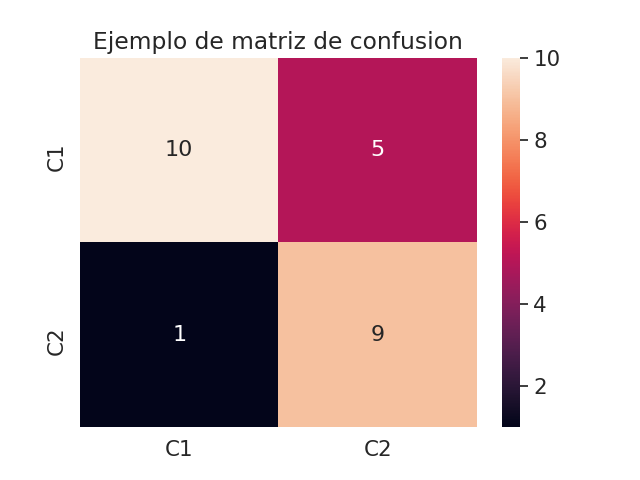
\includegraphics[scale=0.8]{conf_matrix.png}
	\caption{Ejemplo de matriz de confusión}
	\label{fig:conf_matrix}
\end{figure}
Aquí podemos ver cuantas muestras de una clase  el modelo predijo como correctas (de la misma clase) y cuantas muestras de una clase predijo como  erróneas (de distinta clase).\\
\linebreak
A partir de la matriz de confusión, se pueden sacar las siguiente métricas:
\[Precision = \frac{TP} {TP + FP}\]
\[Recall = \frac{TP}{TP + FN}\]
\[FPR = \frac{FP}{FP + TN}\]
\[ F1\_score = 2 \times \frac{Precision \times Recall}{Precision + Recall} \]
Intuitivamente, \textbf{Precision} mide la habilidad del modelo de no clasificar como \textbf{positiva} una muestra que es \textbf{negativa}, mientras que \textbf{Recall} mide la habilidad del modelo para clasificar bien todas las muestras positivas.\\
\linebreak
Cabe destacar que se han explicado para el caso de clasificación binaria, pero estas métricas se pueden extender para la clasificación multi-clase y multi-etiqueta.
\subsection{Curva ROC y AUC}
Partiendo de lo explicado sobre la matriz de confusión, la curva ROC (Receiver Operating Characteristic Curve) es un gráfico donde se representa el \textbf{FPR} (False Positive Rate) en el eje \textbf{X} y el \textbf{TPR} (True Positive Rate o Recall) en el eje \textbf{Y}. Se escogen estas métricas debido a la siguiente hipótesis:\\
A medida que incrementamos el ratio de verdaderos positivos, se va a incrementar el ratio de falsos positivos debido a que es más probable que el modelo clasifique como positivo una muestra que no es positiva.
\begin{figure}[H]
	\centering
	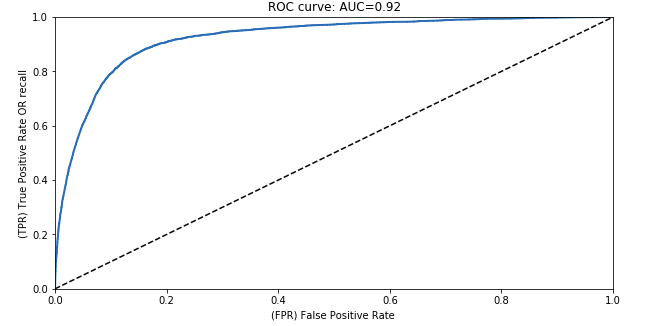
\includegraphics[scale=0.5]{roc}
	\caption{Ejemplo de curva ROC}
	\label{fig:roc}
\end{figure}
Lo ideal, es que la figura se acerque a la esquina superior izquierda lo máximo posible, ya que implicaría que se esta clasificando como correctos todas las muestras positivas y ninguna muestra negativa se está clasificando como positiva.\\
Se puede usar el área bajo la curva  como una métrica para comprobar como de bueno es el modelo. Esta métrica se conoce como \textbf{AUC} (Area Under Curve).\\
\linebreak
Al igual que en regresión (\ref{sec:validation}-\nameref{sec:validation}), se ha usado la técnica de \textit{k-fold validation} para validar el rendimiento de los modelos entrenados.
\section{Modelos de clasificación}
Para clasificación, se van a usar unicamente aquellos modelos que se ha demostrado empíricamente en la sección \ref{sec:algoritmos}-\nameref{sec:algoritmos} que han tenido un buen desempeño. Por tanto se van a usar Árboles de Decisión, Random Forest y SVM.
\subsection{Árboles de Decisión}
En esta sección se va a exponer los resultados obtenidos en clasificación usando  \textbf{Árboles de Decisión}.\\
La siguiente tabla expone los resultados obtenidos:
\begin{figure}[H]
	\centering
	\includegraphics[scale=0.7]{src/dt_cmp_val_metrics}
	\caption{Comparación en conjunto de validación}
	\label{fig:dtre_class_val}
\end{figure}
\begin{figure}[H]
	\centering
	\includegraphics[scale=0.7]{src/dt_cmp_test_metrics}
	\caption{Comparación en conjunto de test}
	\label{fig:dtre_class_testl}
\end{figure}
A continuación, las tablas con los resultados de las métricas y las matrices de confusión obtenidas por los Árboles de decisión usando la categorización usando los rangos $(3.5,5.5,7)$ y $(4,6,7)$
\subsubsection*{Rango $(3.5,5.5,7)$}
\begin{table}[H]
	\centering
	\begin{tabular}{|c|c|c|c|c}
		\cline{1-4}
		FOLD   & F1 Score & AUC Score & Accuracy \\ \cline{1-4}
		Fold 0 & 0.684    & 0.822     & 0.713    \\ \cline{1-4}
		Fold 1 & 0.699    & 0.881     & 0.725    \\ \cline{1-4}
		Fold 2 & 0.691    & 0.84      & 0.713    \\ \cline{1-4}
		Fold 3 & 0.664    & 0.833     & 0.701    \\ \cline{1-4}
		Fold 4 & 0.753    & 0.869     & 0.768    \\ \cline{1-4}
		Fold 5 & 0.698    & 0.849     & 0.724    \\ \cline{1-4}
		Train  & 0.781    & 0.909     & 0.794    \\ \cline{1-4}
		Test   & 0.701    & 0.843     & 0.715    \\ \cline{1-4}
	\end{tabular}
	\caption{Valores de métricas obtenidos usando rango $(3.5,5.5,7)$}
\end{table}

\begin{figure}[H]
	\centering
	\includegraphics[scale=0.5]{src/confusion_matrix_dtree_classification_3-5_5-5_7.png}
	\caption{Matriz de confusión para Árboles de Decisión usando $(3.5,5.5,7)$}
	\label{fig:confusion_matrix_dtree1}
\end{figure}
\subsubsection*{Rango $(4,6,7)$}
\begin{table}[H]
	\centering
	\begin{tabular}{|c|c|c|c|c}
		\cline{1-4}
		FOLD   & F1 Score & AUC Score & Accuracy \\ \cline{1-4}
		Fold 0 & 0.709    & 0.861     & 0.705    \\ \cline{1-4}
		Fold 1 & 0.686    & 0.828     & 0.681    \\ \cline{1-4}
		Fold 2 & 0.698    & 0.842     & 0.697    \\ \cline{1-4}
		Fold 3 & 0.715    & 0.855     & 0.709    \\ \cline{1-4}
		Fold 4 & 0.69     & 0.836     & 0.688    \\ \cline{1-4}
		Fold 5 & 0.7      & 0.844     & 0.696    \\ \cline{1-4}
		Train  & 0.752    & 0.89      & 0.746    \\ \cline{1-4}
		Test   & 0.721    & 0.867     & 0.72     \\ \cline{1-4}
	\end{tabular}
	\caption{Valores de métricas obtenidos usando rango $(4,6,7)$}
\end{table}

\begin{figure}[H]
	\centering
	\includegraphics[scale=0.5]{src/confusion_matrix_dtree_classification_4_6_7}
	\caption{Matriz de confusión para Árboles de Decisión usando $(4,6,7)$}
	\label{fig:confusion_matrix_dtree2}
\end{figure}
\pagebreak
\subsection{Random Forest}
En esta sección se va a exponer los resultados obtenidos en clasificación usando  \textbf{Random Forest}.
A continuación se muestran una serie de gráficos comparando las distintas métricas que se han seleccionado:
\begin{figure}[H]
	\centering
	\includegraphics[scale=0.5]{src/rf_class_cmp_val_metrics}
	\caption{Comparación en conjunto de validación}
	\label{fig:rf_class_cmp_val}
\end{figure}

\begin{figure}[H]
	\centering
	\includegraphics[scale=0.5]{src/rf_class_cmp_test_metrics}
	\caption{Comparación en conjunto de test}
	\label{fig:rf_class_cmp_test}
\end{figure}
En las secciones siguientes, se va a mostrar las tablas con los valores de métricas obtenidas por Random Forest y las matrices de confusión correspondientes.
\subsubsection*{Rango $(3,5,7)$}
\begin{table}[H]
	\centering
	\begin{tabular}{|c|c|c|c|c}
		\cline{1-4}
		FOLD   & F1 Score & AUC Score & Accuracy \\ \cline{1-4}
		Fold 0 & 0.694    & 0.858     & 0.721    \\ \cline{1-4}
		Fold 1 & 0.755    & 0.898     & 0.769    \\ \cline{1-4}
		Fold 2 & 0.699    & 0.883     & 0.717    \\ \cline{1-4}
		Fold 3 & 0.693    & 0.867     & 0.709    \\ \cline{1-4}
		Fold 4 & 0.748    & 0.892     & 0.776    \\ \cline{1-4}
		Fold 5 & 0.718    & 0.88      & 0.738    \\ \cline{1-4}
		Train  & 0.993    & 1.0       & 0.994    \\\cline{1-4}
		Test   & 0.739    & 0.885     & 0.761    \\ \cline{1-4}
	\end{tabular}
	\caption{Valores de métricas obtenidos usando rango $(3,5,7)$}
\end{table}
\begin{figure}[H]
	\centering
	\includegraphics[scale=0.5]{src/confusion_matrix_rf_class_3_5_7.png}
	\caption{Matriz de confusión para Random Forest usando $(3,5,7)$}
	\label{fig:confusion_matrix_rf1}
\end{figure}

\subsection*{Rango $(4,6,7)$}
\begin{table}[H]
	\centering
	\begin{tabular}{|c|c|c|c|c}
		\cline{1-4}
		FOLD   & F1 Score & AUC Score & Accuracy \\ \cline{1-4}
		Fold 0 & 0.702    & 0.887     & 0.701    \\  \cline{1-4}
		Fold 1 & 0.72     & 0.884     & 0.713    \\  \cline{1-4}
		Fold 2 & 0.763    & 0.903     & 0.765    \\  \cline{1-4}
		Fold 3 & 0.747    & 0.891     & 0.745    \\  \cline{1-4}
		Fold 4 & 0.703    & 0.868     & 0.696    \\  \cline{1-4}
		Fold 5 & 0.727    & 0.887     & 0.724    \\  \cline{1-4}
		Train  & 0.998    & 1.0       & 0.998    \\ \cline{1-4}
		Test   & 0.748    & 0.901     & 0.746    \\ \cline{1-4}
	\end{tabular}
	\caption{Valores de métricas obtenidos usando rango $(4,6,7)$}
\end{table}
\begin{figure}[H]
	\centering
	\includegraphics[scale=0.5]{src/confusion_matrix_rf_class_4_6_7.png}
	\caption{Matriz de confusión para Random Forest usando $(4,6,7)$}
	\label{fig:confusion_matrix_rf2}
\end{figure}
\pagebreak
\subsection{Support Vector Machines}
En esta sección se va a exponer los resultados obtenidos en clasificación usando  \textbf{Random Forest}.\\
La siguiente tabla expone los resultados obtenidos:
En esta sección se va a exponer los resultados obtenidos en clasificación usando  \textbf{Random Forest}.
A continuación se muestran una serie de gráficos comparando las distintas métricas que se han seleccionado:
\begin{figure}[H]
	\centering
	\includegraphics[scale=0.5]{src/svc_cmp_val_metrics.png}
	\caption{Comparación en conjunto de validación}
	\label{fig:svc_class_cmp_val}
\end{figure}

\begin{figure}[H]
	\centering
	\includegraphics[scale=0.5]{src/svc_cmp_test_metrics.png}
	\caption{Comparación en conjunto de test}
	\label{fig:svc_class_cmp_test}
\end{figure}
En las secciones siguientes, se va a mostrar las tablas con los valores de métricas obtenidas por Random Forest y las matrices de confusión correspondientes.
\subsubsection*{Rango $(3.5,5.5,7)$}
\begin{table}[H]
	\centering
	\begin{tabular}{|c|c|c|c|c}
		\cline{1-4}
		FOLD   & F1 Score & AUC Score & Accuracy \\ \cline{1-4}
		Fold 0 & 0.682    & 0.846     & 0.717    \\ \cline{1-4}
		Fold 1 & 0.713    & 0.887     & 0.753    \\ \cline{1-4}
		Fold 2 & 0.729    & 0.899     & 0.749    \\ \cline{1-4}
		Fold 3 & 0.698    & 0.861     & 0.713    \\ \cline{1-4}
		Fold 4 & 0.735    & 0.91      & 0.772    \\ \cline{1-4}
		Fold 5 & 0.711    & 0.881     & 0.741    \\ \cline{1-4}
		Train  & 0.928    & 0.989     & 0.933    \\ \cline{1-4}
		Test   & 0.712    & 0.887     & 0.742    \\ \cline{1-4}
	\end{tabular}
	\caption{Valores de métricas obtenidos usando rango $(3.5,5.5,7)$}
\end{table}
\begin{figure}[H]
	\centering
	\includegraphics[scale=0.5]{src/confusion_matrix_svc_3-5_5-5_7.png}
	\caption{ confusión para SVM usando $(3.5,5.5,7)$}
	\label{fig:confusion_matrix_svm1}
\end{figure}

\subsubsection*{Rango $(4,6,7)$}
\begin{table}[H]
	\centering
	\begin{tabular}{|c|c|c|c|c}
		\cline{1-4}
		FOLD   & F1 Score & AUC Score & Accuracy \\ \cline{1-4}
		Fold 0 & 0.65     & 0.856     & 0.649    \\  \cline{1-4}
		Fold 1 & 0.702    & 0.886     & 0.705    \\  \cline{1-4}
		Fold 2 & 0.742    & 0.88      & 0.745    \\  \cline{1-4}
		Fold 3 & 0.739    & 0.888     & 0.741    \\  \cline{1-4}
		Fold 4 & 0.681    & 0.862     & 0.676    \\  \cline{1-4}
		Fold 5 & 0.703    & 0.874     & 0.703    \\  \cline{1-4}
		Train  & 0.918    & 0.991     & 0.917    \\  \cline{1-4}
		Test   & 0.714    & 0.881     & 0.718    \\  \cline{1-4}
	\end{tabular}
	\caption{Valores de métricas obtenidos usando rango $(4,6,7)$}
\end{table}
\begin{figure}[H]
	\centering
	\includegraphics[scale=0.5]{src/confusion_matrix_svc_4_6_7.png}
	\caption{Matriz de confusión para SVM usando $(4,6,7)$}
	\label{fig:confusion_matrix_svc2}
\end{figure}

\subsection{Conclusiones}
Como se puede apreciar, ninguno de los algoritmos no han tenido problemas clasificando la clase \textbf{IEAlta}, clasificando correctamente más del $80\%$ de las instancias de esta clase.
Los algoritmos han tenido más problemas a la hora de clasificar correctamente la clase \textbf{IEBaja}, clasificando correctamente solo el $50\%$. Volviendo a la figura \ref{tab:ocurrencia_valores} donde se mostraba el conteo de clases, se puede apreciar que la clase formada por los valores más bajos tiene una menor cantidad de muestras, explicando así que los algoritmos fallen más comúnmente en estas clases, clasificando una gran parte como \textbf{IEMedia} (tiene sentido ya que es la clase más 'cercana') .
Por

	\pagebreak

	\newpage
	\nocite{*}

	\bibliography{bibliografia}
	\bibliographystyle{plain}

\end{document}
